
%%==================================================
%% demo.tex for BIT Thesis
%% modified by yang yating
%% version: 1.2
%% last update: Jan. 4th, 2018
%%==================================================

% 默认单面打印 oneside 、硕士论文模板 master

\documentclass[oneside, master]{BIT-thesis-grd}
% 模板选项: 硕士论文 master; 博士论文 doctor

%==============更改数学字体设置,Latin Modern Math 默认的的确有点细,看个人需要,下面提供一种方法,需要的可以取消注释=========%

% \usepackage[bold-style=ISO]{unicode-math} %采用unicode-math,可以直接输入Unicode公式,当然传统的输入就行
% \setmathfont{XITS Math}  %目前unicode-math 支持几种数学字体,具体用法可以查看帮助文档,这里采用类似times字体科学数学字体,可以取消注释对比
\usepackage[ruled,linesnumbered]{algorithm2e}
\usepackage{tikz}
\usepackage{pgfplots}
\pgfplotsset{compat=1.18}

\begin{document}
%%%%%%%%%%%%%%%%%%%%%%%%%%%%%%
%% 封面
%%%%%%%%%%%%%%%%%%%%%%%%%%%%%%

% 中文封面内容(关注内容而不是表现形式)
\classification{TQ028.1}
\UDC{540}

\title{ReL4:高性能异步微内核设计与实现}
\vtitle{ReL4:高性能异步微内核设计与实现}
\author{廖东海}
\institute{计算机学院}
\advisor{陆慧梅}
\chairman{***}
\degree{工学硕士}
\major{计算机科学与技术}
\school{北京理工大学}
\defenddate{****年*月}
%\studentnumber{**********}


% 英文封面内容(关注内容而不是表现形式)
\englishtitle{ReL4: Design and Implementation of High-performance Asynchronous Microkernel}
\englishauthor{Liao Donghai}
\englishadvisor{Lu Huimei}
\englishchairman{***}
\englishschool{Beijing Institute of Technology}
\englishinstitute{****}
\englishdegree{****}
\englishmajor{****}
\englishdate{*,****}

% 封面绘制
\maketitle

%打印竖排论文题目
\makeVerticalTitle

% 中文信息
\makeInfo

% 英文信息
\makeEnglishInfo

% 论文原创性声明和使用授权
\makeDeclareOriginal

%%%%%%%%%%%%%%%%%%%%%%%%%%%%%%
%% 前置部分
%%%%%%%%%%%%%%%%%%%%%%%%%%%%%%
\frontmatter

% 摘要
%%==================================================
%% abstract.tex for BIT Master Thesis
%% modified by yang yating
%% version: 0.1
%% last update: Dec 25th, 2016
%%==================================================

\begin{abstract}

微内核将大部分系统服务运行在用户空间,相比于宏内核有更好的稳定性、扩展性和内核安全性,在微内核系统中,应用程序通过进程间通信(IPC)而非系统调用来请求服务,频繁的IPC造成的特权级切换将产生巨大开销,成为了系统的性能瓶颈。以seL4为代表的现代微内核将同步IPC作为主要通信手段,并以异步通知机制作为辅助手段来提升系统并发度,这些机制在一定程度上减少了IPC的开销,提升了系统性能,然而它们在设计上仍有三点不足:1)在支持同步IPC的情况下冗余地支持了异步通知机制,这违反了内核最小化原则;2)通知机制依赖内核的转发,会造成大量的特权级切换;3)系统调用和同步IPC会导致无关请求顺序执行,无法充分利用硬件资源。

针对以上三点缺陷,本文设计并实现了ReL4——一套异步化的高性能微内核架构,其主要设计理念是将异步通知机制作为内核支持的唯一通信手段,在用户态通过共享缓冲区实现IPC的数据传递,并通过通知机制进行同步,保证了内核最小化原则;同时ReL4基于用户态中断,在兼容seL4接口的基础上,设计了无需内核转发的U-notification机制,避免了通知机造成的大量特权级切换;最后,ReL4通过异步运行时来实现异步IPC和异步系统调用,避免了无关IPC和系统调用请求的顺序执行,在充分利用硬件资源,提升系统并发度的同时,提升系统易用性。

本文在FPGA上实现了ReL4的原型系统,将U-notification、异步IPC和异步系统调用分别与seL4进行了对比测试,并评估了真实的TCP Server在ReL4的性能表现。测试结果表明,相比于seL4,ReL4能够大幅减少系统中特权级切换的次数,在低并发场景下有着接近的性能,在高并发场景下拥有更卓越的表现,从而证明了ReL4架构的可行性和优越性。

\keywords{微内核; 异步; 进程间通信; 用户态中断}
\end{abstract}  

\begin{englishabstract}
The microkernel runs most system services in the user space. Compared with the monolithic kernel, it has better stability, extensibility, and kernel security. In a microkernel system, applications request services through inter-process communication (IPC) instead of system calls. The frequent privilege level switches caused by IPC generate huge overheads, which become a performance bottleneck of the system. Modern microkernels represented by seL4 use synchronous IPC as the main communication means and adopt an asynchronous notification mechanism as an auxiliary means to improve the system concurrency. These mechanisms reduce the IPC overhead to a certain extent and enhance the system performance. However, there are still three design deficiencies: (1) The asynchronous notification mechanism is redundantly supported while synchronous IPC is supported, which violates the principle of kernel minimization; (2) The notification mechanism relies on the forwarding of the kernel, resulting in a large number of privilege level switches; (3) System calls and synchronous IPC will cause irrelevant requests to be executed sequentially, failing to fully utilize hardware resources.

Aiming at the above three defects, this paper designs and implements ReL4, a set of asynchronous high-performance microkernel architecture. Its main design concept is to use the asynchronous notification mechanism as the only communication means supported by the kernel. In the user space, the data transfer of IPC is realized through a shared buffer, and synchronization is carried out through the notification mechanism, ensuring the principle of kernel minimization. At the same time, based on user-space interrupts and on the basis of being compatible with the seL4 interface, ReL4 designs the U-notification mechanism that does not require kernel forwarding, avoiding a large number of privilege level switches caused by the notification mechanism. Finally, ReL4 implements asynchronous IPC and asynchronous system calls through an asynchronous runtime, avoiding the sequential execution of irrelevant IPC and system call requests. While fully utilizing hardware resources and improving system concurrency, it also enhances the usability of the system.

This paper implements a prototype system of ReL4 on an FPGA. The U-notification, asynchronous IPC, and asynchronous system calls are respectively compared and tested with seL4, and the performance of a real TCP Server on ReL4 is evaluated. The test results show that compared with seL4, ReL4 can significantly reduce the number of privilege level switches in the system, has a similar performance in low-concurrency scenarios, and has more excellent performance in high-concurrency scenarios, thus proving the feasibility and superiority of the ReL4 architecture.

\englishkeywords{microkernel; asynchronous; inter-process communication; user-mode interrupt }

\end{englishabstract}

%% 符号对照表,可选,如不用可注释掉
% 加入目录
\tableofcontents


%加入图、表索引(同时取消图表索引中章之间的垂直间隔)
\let\origaddvspace\addvspace
\renewcommand{\addvspace}[1]{}
\listoffigures
\listoftables
\renewcommand{\addvspace}[1]{\origaddvspace{#1}}

\begin{denotation}
	
\item[BIT] 北京理工大学的英文缩写
\item[\LaTeX] 一个很棒的排版系统
\item[\LaTeXe] 一个很棒的排版系统的最新稳定版
\item[\XeTeX] \LaTeX{}的好兄弟,事实上他有很多个兄弟,但是这个兄弟对各种语言的支持能力都很强
\item[ctex] 成套的中文\LaTeX{}解决方案,由一帮天才们开发
\item[\ce{H2SO4}] 硫酸
\item[$ e^{\pi{}i}+1=0$] 一个集自然界五大常数一体的炫酷方程
\item[\ce{2H2 + O2 -> 2H2O}] 一个昂贵的生成生命之源的方程式

\end{denotation}


%%%%%%%%%%%%%%%%%%%%%%%%%%%%%%
%% 正主体部分
%%%%%%%%%%%%%%%%%%%%%%%%%%%%%%
\mainmatter

%% 各章正文内容
%%==================================================
%% chapter01.tex for BIT Master Thesis
%% modified by yang yating
%% version: 0.1
%% last update: Dec 25th, 2016
%%==================================================
\chapter{绪论}
\label{chap:intro}
\section{课题研究的背景和意义}

随着科技的发展,微内核广泛应用于工控系统、嵌入式系统等领域\cite{rana2023survey}。相比于宏内核,微内核将内存管理、设备驱动、文件系统等与核心功能分离,运行在用户空间,这种隔离机制使得单个服务的故障不会直接影响到内核和其他服务,从而提升了系统的整体稳定性\cite{Thallapally2024};微内核通过精简核心功能,减少攻击面,从而提升内核安全性\cite{heiser2008role};此外,模块化的设计使得系统更易于维护和升级\cite{herder2006construction}。在微内核系统中,应用程序通过进程间通信(IPC) 而非系统调用来请求服务,这或许能够满足早期性能不敏感的软件需求,然而在对软件性能有着更高要求的今天,频繁IPC造成的特权级切换将产生巨大开销,成为系统的性能瓶颈\cite{liedtke1996toward}。

30 年前 Liedtke 提出的L4 \cite{liedtke1993improving} 重新设计了微内核系统,通过组合系统调用、快速路径、消息寄存器等优化手段,从硬件层到软件层对IPC进行了系统性优化,证明了微内核的IPC 也可以很快\cite{jochen1994mu},之后以seL4 \cite{klein2009sel4} 为代表的现代微内核的 IPC 框架也基本延续了 L4 的设计理念,以同步 IPC作为主要的通信方式。然而同步IPC迫使单线程中上下文无关的请求以顺序的形式执行,系统只能通过多线程实现并发,而为了更好地利用硬件资源,现代微内核大多引入异步的通知机制来简化并发程序设计,提升多核的利用率,这违反了微内核的最小化设计原则,增加了内核的复杂性。

而随着软件复杂性的提升,用户希望系统级软件如数据库管理系统、网络服务器等能够快速处理大量系统调用和IPC\cite{Caruso2021},而微内核将操作系统的大部分服务(如网络协议栈、文件系统等)移到用户态,从而使得IPC数量和频率激增,特权级切换成为性能瓶颈。此外,新出现的硬件漏洞如Meltdown\cite{lipp2020meltdown}和Spectre\cite{kocher2020spectre} 漏洞促使内核使用 KPTI补丁\cite{kernel_pti}来分离用户程序和内核的页表,进一步增加了陷入内核的开销。最后,现代微内核的外设驱动往往存在于用户态,外设中断被转化为异步通知,需要用户态驱动主动陷入内核来进行接收,这在一定程度上成为了外设驱动的性能瓶颈\cite{blackham2012improving}。综上所述,由IPC和通知机制引起的特权级切换已经成为制约系统性能的主要因素。

本文提出ReL4,一个用Rust编写的高性能异步微内核,它将同步IPC从内核中移除,基于用户态中断技术设计了无需陷入内核的U-notification机制,在兼容capability机制的基础上改造微内核的通知机制,并利用改造后的U-notification和异步化编程设计和实现了一套绕过内核的异步IPC和异步系统调用框架。ReL4在设计理念上将内核最小化原则贯彻得更加彻底,并通过软硬件协同的方式进一步提升微内核的IPC性能,为下一代微内核的发展指出一个可能的方向。

\section{国内外研究现状及发展趋势}
%\label{sec:***} 可标注label

\subsection{微内核IPC的发展现状}
%\label{sec:features}

现代微内核的进程间通信(IPC)优化研究可追溯至Liedtke提出的L4微内核架构。针对早期微内核IPC存在的性能瓶颈问题,L4从硬件抽象层、系统架构设计和软件接口规范等多个维度进行了系统性重构。这些优化措施主要可归纳为内核执行路径优化和上下文切换优化两个关键方向。

在内核执行路径优化方面,L4通过物理消息寄存器来传递短消息,有效规避了短消息场景下的内存拷贝开销。然而,随着存储器访问性能的持续提升,这种零拷贝优化带来的相对收益逐渐减弱。更为关键的是,物理寄存器的硬件依赖性导致平台移植困难,并可能干扰编译器的寄存器分配优化\cite{heiser2016l4}。这一局限性促使现代微内核普遍转向虚拟消息寄存器方案。对于长消息传输,L4采用临时内存映射机制避免数据拷贝,但该设计增加了内核处理缺页异常的复杂度\cite{heiser2016l4},因而被后续系统所摒弃。值得注意的是,L4针对高频IPC场景设计了专门的快速路径(fast-path)机制\cite{peng2020fast}(如图\ref{fig:fast-path}所示),通过简化参数解析和任务调度流程提升性能。然而,该优化对消息长度和任务优先级等参数有严格约束,且难以扩展至多核环境。

\begin{figure*}[htbp]
    \centering
    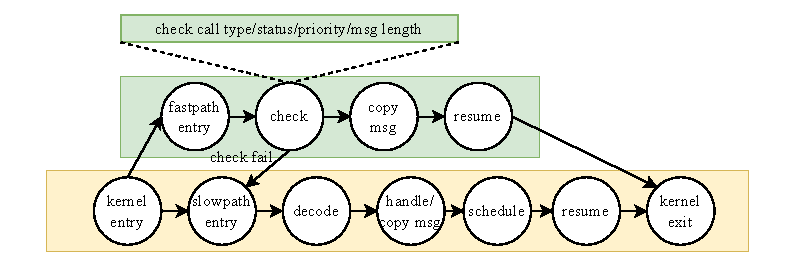
\includegraphics[width=1.0\textwidth]{figures/fast-path.drawio.pdf}
    \caption{fast-path优化示意图}\label{fig:fast-path}
\end{figure*}

在特权级切换优化方面,L4进行了多项开创性探索。虽然其物理消息寄存器方案确实降低了上下文切换开销,但前文所述的局限性最终导致该设计被虚拟寄存器方案取代\cite{heiser2016l4}。L4的其中一个创新性贡献在于发现了IPC通信中普遍存在的客户端-服务器模式特征,并据此设计了组合式系统调用接口:将Send+Reply整合为Call操作,将Reply+Recv合并为ReplyRecv操作。这种设计显著减少了特权级切换频率,至今仍是现代微内核的标准优化手段。此外,L4采用地址空间标识符(ASID)机制来缓解TLB冲刷问题\cite{arm2009asid},通过维护进程专属的快表项降低了上下文切换带来的性能损耗。然而,这些优化仍无法完全消除特权级切换导致的TLB污染和缓存失效问题\cite{cox2017efficient}。

除此之外,L4仅支持同步IPC,对于多核架构,同步IPC会导致服务调用被顺序执行,导致资源浪费\cite{kuang2013towards}。其次,同步IPC强制用户态以多线程的形式处理并发请求,导致了线程同步的复杂性。现代微内核在内核中引入异步通知机制,简化并发编程模型,却使得内核功能冗余,违反了内核最小化原则。

总而言之,现代微内核在单核环境下的IPC内核路径上的优化已经较为完善,在最理想的情况下仅需要两次特权级切换,然而对多核环境下,由于需要核间中断,IPC无法进入快速路径,导致多核下的IPC内核路径依旧冗长。而现代微内核在特权级切换的优化方面仍然停留缓解的层面上,导致特权级切换会成为IPC的性能瓶颈。

\subsection{特权级切换}
特权级切换带来的性能开销可分解为直接和间接两个部分\cite{li2007quantifying}。直接开销主要体现为上下文保存与恢复所需的额外指令执行周期,而间接开销则源于地址空间切换导致的缓存污染效应\cite{gotzfried2017cache},这种效应会显著降低后续指令的执行效率。如表\ref{tab:seL4_call_cost}所示,基于FPGA平台的实测数据表明,在seL4微内核中执行一次Call IPC操作时,地址空间切换所产生的时间开销占比最高,其次是上下文切换和fast-path检查过程。特别值得注意的是,当fast-path检查未通过时,系统将转入slow-path处理流程,该流程涉及更复杂的消息解码和任务调度机制,会进一步加剧IPC性能的下降。针对这一关键性能瓶颈问题,学术界和工业界已从硬件架构优化和软件算法改进等多个维度展开了广泛而深入的研究探索。
\begin{table}
    \centering
    \caption{seL4一次IPC中各操作的开销占比}
    \begin{tabular}{|c|c|}
        \hline 
        操作 & 占比 \\
        \hline
        保存和恢复上下文 & 14.5\% \\
        \hline
        地址空间切换 & 59.4\% \\
        \hline
        fast - path检查 & 20.1\% \\
        \hline
        消息拷贝 & 1.5\% \\
        \hline
        其他 & 4.5\% \\
        \hline
    \end{tabular}
    \label{tab:seL4_call_cost}
\end{table}
    
从硬件出发的角度出发,大多数工作通过设计特殊的硬件或者特殊的指令来绕过内核实现IPC。如SkyBridge\cite{mi2019skybridge}允许进程在IPC中直接切换到目标进程的虚拟地址空间并调用目标函数,它通过精心设计一个Root Kernel提供虚拟化的功能,通过VMFUNC地址空间的直接切换\cite{li2015reducing},并通过其他一系列软件手段来保证安全性,但这种方案仅适用于虚拟化环境中。XPC\cite{du2019xpc}则直接使用硬件来提供一个无需经过内核的同步功能调用,并提供一种新的空间映射机制用于调用者与被调用者之间的零拷贝消息传递,然而该方案没有相应的硬件标准,也没有一款通用的处理器对其进行支持。这些方法都基于特殊的环境或者没有标准化的硬件来实现,适用范围有限。

从软件出发的角度出发,相关工作主要分为两类:第一类方法通过将用户态和内核态的功能扁平化来减少内核与用户态的切换开销,如unikernel\cite{kuo2020linux, olivier2019binary, yu2017web}将所有用户态代码都映射到内核态执行,Userspace Bypass\cite{zhou2023userspace} 通过动态二进制分析将两个系统调用之间的用户态代码移入内核态执行,从而减少陷入内核的次数,kernel bypass\cite{jeong2014mtcp, yang2017spdk}则通过将硬件驱动(传统内核的功能)移入用户态,从而减少上下文的切换。这些方法要么需要特殊的硬件支持,要么难以与微内核的设计理念兼容。第二类方法则是允许用户空间对多个系统调用请求排队,并通过一次提交将他们注册给内核,如FlexSC\cite{soares2010flexsc}通过在用户态设计一个用户态线程的运行时,将用户态线程发起的系统调用自动收集,然后陷入内核态进行批量执行。该方法虽然可以有效的减少陷入内核的次数,但如何设置提交的时机难以把握,过短的提交间隔将导致切换次数增加,过长的提交间隔则会导致CPU空转。

虽然现有工作难以广泛且有效地应用到微内核中,但他们的思路值得借鉴,他们的缺陷驱使研究者去寻求更好的方案。在硬件方面,一种新型的硬件技术方案——用户态中断\cite{nassif2022sapphire, RISCVPrivileged2020}逐渐被各个硬件平台(x86,RISC-V)采纳,它通过在CPU中新增中断代理机制和用户态中断的状态寄存器,当中断代理机制检测到状态寄存器发生变化时,会将中断以硬件转发的形式传递给用户态程序,从而绕过内核。该硬件方案已经在Sapphire Rapids x86处理器上和RISCV的N扩展中有了一定的支持,适用范围更加广泛。而在软件方面,异步被广泛用于请求合并和开销均摊,传统类Unix系统提供的类似select IO多路复用接口相对简陋,迫使用户态代码采用事件分发的编程范式来处理异步事件,代码相对复杂,可读性较弱。而新兴的Rust\cite{levy2015ownership, balasubramanian2017system}语言对异步有着良好的支持,其零成本抽象的设计也让它作为系统编程语言有着强大的竞争力。使用Rust进行内核和用户态基础库的开发,可以更好地对异步接口进行抽象,改善接口的易用性和代码的可读性。

\begin{table}
    \centering
    \caption{国内外研究现状汇总}
    \resizebox{\textwidth}{!}{ % \textwidth 表示文本宽度,! 表示保持宽高比
    \begin{tabular}{|c|c|c|c|}
        \hline
        \textbf{优化方法} & \textbf{详细分类} & \textbf{实例} & \textbf{缺点} \\
        \hline
        \multirow{3}{*}{减少内核路径} & 临时地址映射 & \cite{liedtke1993improving} & \multirow{3}{*}{上下文切换开销已经成为性能瓶颈} \\
        \cline{2-3}
         & 快速路径 & \multirow{2}{*}{\cite{liedtke1993improving, klein2009sel4, heiser2010okl4, smejkal2015transactional}} & \\
        \cline{2-2}
         & 消息寄存器 & & \\
        \hline
        \multirow{5}{*}{减少上下文切换开销} & 消息寄存器 & \multirow{2}{*}{\cite{liedtke1993improving, klein2009sel4, heiser2010okl4, smejkal2015transactional}} & \multirow{4}{*}{无法从根本上消除切换开销} \\
        \cline{2-2} \cline{4-4}
         & 组合系统调用 & & \\
        \cline{2-3}
         & ASID机制 & \cite{klein2009sel4} & \\
        \cline{2-4}
         & 统一地址空间 & \cite{kuo2020linux, olivier2019binary, yu2017web, zhou2023userspace, jeong2014mtcp, yang2017spdk} & \multirow{2}{*}{与微内核设计理念相悖,无法有效地实施到微内核中} \\
        \cline{2-3}
         & 批量系统调用 & \cite{soares2010flexsc} & \\
        \hline
        \multirow{3}{*}{硬件优化} & 虚拟化指令 & \cite{mi2019skybridge} & 仅适用于虚拟化环境 \\
        \cline{2-4}
         & \multirow{2}{*}{直接硬件辅助} & \cite{du2019xpc} & 没有硬件标准,没有通用硬件的支持 \\
        \cline{3-4}
         & & \cite{mehta2021x86, pintouser} & --- \\
        \hline
        \end{tabular}
    }
    \label{tab:optimization_methods}
\end{table}

\subsection{Rust语言与异步编程机制}
在现代计算机系统中,随着多任务处理和并发编程的普及\cite{rights2005software},程序需要处理的任务越来越复杂,任务之间的依赖关系也变得越来越松散。传统的同步机制,即任务按照严格的顺序执行,前一个任务完成后才能开始后一个任务,已经无法满足高效处理多个并发任务的需求\cite{adya2002cooperative}。因此,异步机制应运而生\cite{deligiannis2015asynchronous},它允许任务在不阻塞其他任务的情况下执行,从而提高了系统的整体性能和响应速度。传统操作系统大多使用C语言作为主要语言来实现异步\cite{bovet2005understanding},用于应对内核场景下的复杂场景,其虽然相对灵活,但也存在一些固有缺陷:
\begin{itemize}
    \item 编程困难:异步编程需要在代码中处理多个任务之间的协作和同步,这增加了编程的复杂性。开发者需要仔细考虑异步任务之间的依赖关系、执行顺序以及错误处理,可能导致代码难以理解和维护。
    \item 调试困难:异步编程的执行流程是非线性的,这增加了调试的难度。由于异步任务可能在不同时间点触发和执行,调试时需要跟踪多个任务的状态和交互,使得调试过程更加繁琐和耗时。
    \item 代码可读性下降:异步编程通常涉及回调函数、事件监听等结构,这些结构可能导致代码的可读性下降。回调函数的嵌套使用(即“回调地狱”)可能使代码结构变得混乱,难以阅读和理解。
    \item 代码可维护性下降:异步编程中的任务依赖关系和同步机制可能随着代码的发展而变得更加复杂,这增加了代码维护的难度。当需要修改或添加新的异步任务时,开发者需要仔细考虑对现有代码的影响,并确保新任务与现有任务之间的正确同步和协作。
  \end{itemize}

而相对高阶的语言提供了对异步的原生支持,如C++\cite{belson2020c}和Rust\cite{kroning2023concurrency},在语言层面对异步编程提供了支持,不依赖操作系统以及标准库,有着良好的移植性和兼容性。本节我们将介绍Rust语言对异步的支持\cite{matsakis2018async}。

Rust语言的异步编程模型体现了一种系统级的创新设计,其核心思想是通过编译时状态机转换来实现高效的异步执行\cite{samson2024asynchronous}。该模型建立在Future这一基础抽象之上,Future trait定义的poll机制采用了一种独特的延迟执行模式,这种设计使得异步任务能够被精确控制,而非传统的事件回调模式\cite{edwards2009coherent}。值得注意的是,Rust的异步机制通过编译器生成的状态机转换,在保证零成本抽象的同时\cite{tjader2021rtic},实现了与手动优化代码相当的性能表现。

在运行时支持方面,Rust采用了模块化的设计哲学\cite{klabnik2020rust}。异步运行时被明确划分为Executor和Reactor两个核心组件\cite{moslehianexperimental},这种关注点分离的设计带来了显著的架构优势。Executor负责调度逻辑,而Reactor处理I/O事件通知,二者的协同工作通过高效的wake机制实现。特别值得关注的是,Rust的标准库刻意不绑定特定的运行时实现\cite{rust2021std},这种设计决策赋予了开发者根据应用场景选择最优运行时的灵活性。从系统编程的角度看,这种模块化设计使得异步Rust能够适应从嵌入式系统到分布式服务的各种应用场景。

语言层面的async/await语法为异步编程提供了重要的工程实践支持\cite{matsakis2018async}。这一语法糖不仅大幅提升了代码的可读性和可维护性,更重要的是,它使得编译器能够进行深度的优化。通过将异步控制流转换为状态机,Rust实现了与手动编写回调代码相当的性能,同时避免了回调地狱等常见的异步编程陷阱\cite{edwards2009coherent}。从类型系统的角度来看,async函数返回的Future保持了严格的类型约束,这使得编译器能够在编译期捕获大量潜在的逻辑错误,显著提升了异步代码的可靠性。

此外,Rust语言的设计哲学与微内核架构在系统安全性和可靠性方面展现出深刻的协同效应。从内存管理机制来看,Rust的所有权系统通过编译时的严格检查\cite{levy2015ownership},为微内核的关键组件提供了静态的内存安全保障。这种编译期验证机制与微内核最小化特权域的设计原则高度契合,使得内核开发者能够在保证性能的前提下,有效预防各类内存安全漏洞。

基于上述工程实践考量,本文选择Rust作为ReL4微内核的主要实现语言。这一选择不仅能够充分利用Rust在系统编程领域的独特优势,更重要的是,Rust的现代化语言特性为构建安全、高效的异步微内核提供了更加理想的开发工具链。

\subsection{用户态中断与TAIC加速器}

现代处理器通过多特权级设计实现安全隔离\cite{waterman2016riscv},但特权级切换带来的性能开销已成为系统优化的关键瓶颈。传统的中断处理机制依赖于内核介入\cite{bovet2005understanding},导致频繁的特权级切换和上下文保存恢复操作,不仅产生直接的指令执行开销,还会因页表切换和缓存失效引入显著的间接性能损失\cite{gotzfried2017cache}。

\begin{figure*}[htbp]
    \centering
    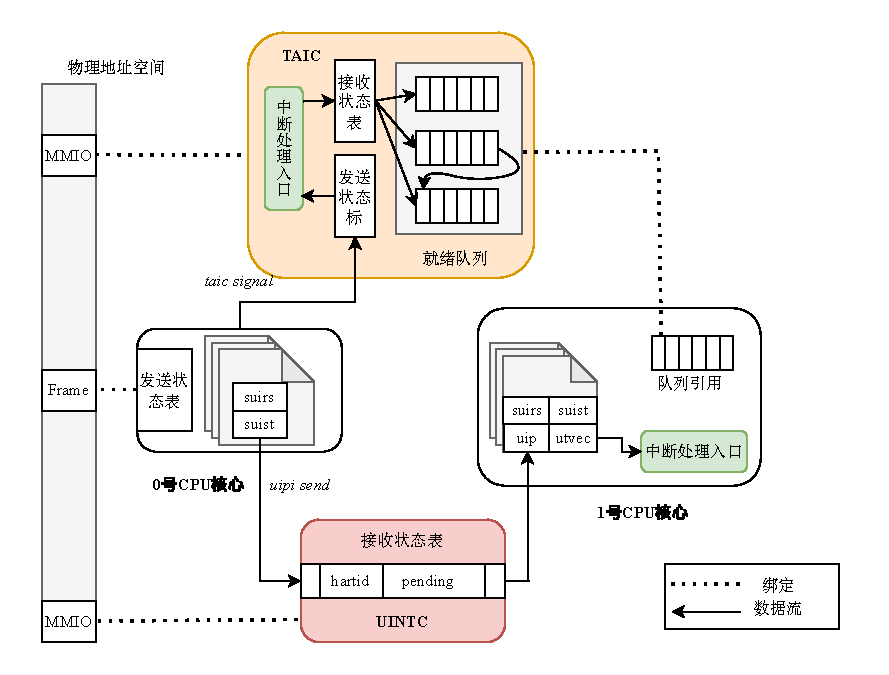
\includegraphics[width=1.0\textwidth]{figures/uintc_taic.pdf}
    \caption{用户态中断和TAIC加速器的示意图}\label{fig:uintc_taic}
\end{figure*}

为降低这一开销,用户态中断(User-Level Interrupt)\cite{mehta2021x86}机制应运而生。该技术通过在CPU中引入中断代理和专用状态寄存器,使中断能够直接在用户态处理,完全绕过内核参与。以RISC-V N扩展的实现为例,如\ref{fig:uintc_taic}所示,用户态中断的核心创新在于将中断状态管理分为操作系统维护的发送状态表和硬件控制器(UINTC)管理的接收状态表。当触发中断时,硬件通过专用指令自动完成状态查询和处理器间中断传递,最终直接跳转到用户态注册的处理函数执行。这一设计不仅消除了内核转发的软件开销,还保持了良好的缓存局部性。


在UINTC基础上的进一步优化催生了任务感知中断控制器(TAIC)\cite{taic_github}。与基础用户态中断相比,TAIC的创新性体现在两个方面:首先,它将所有状态表统一交由硬件管理,通过MMIO寄存器访问替代内存查表操作,减少了中断发送阶段的内存访问延迟;其次,该控制器深度整合了任务调度功能,能够在中断到达时自动将预注册的处理任务加入硬件就绪队列,完全消除了软件唤醒的开销。这种硬件-软件协同设计使得中断处理流程更加高效,在保持用户态执行优势的同时,进一步减少了CPU执行流的打断频率,为实时性要求高的应用场景提供了更优的解决方案。

从系统架构演进的角度看,从传统内核中断到用户态中断,再到任务感知中断控制器的发展,体现了中断处理机制从软件主导到硬件加速的转变趋势\cite{song2021hardware}。这种转变不仅降低了中断延迟,更重要的是通过硬件原语支持,为构建更高效的异步任务处理框架奠定了基础。


\section{主要研究内容}
本文以免费开源的seL4的IPC系统主要研究对象,介绍了seL4中IPC的设计细节以及相关设计缺陷,针对seL4的相关缺陷,基于用户态中断,给出了高性能异步微内核的整体设计方案,包含了无需内核转发的通知机制U-notification、异步IPC与异步系统调用,并基于Rust语言在RISC-V平台实现了ReL4原型系统。在FPGA上将U-notification、异步IPC 和异步系统调用分别与seL4进行了对比测试,并评估了ReL4在真实的TCP Server Benchmark上的性能表现。论文内容结构安排如下:

第1章,绪论部分,阐述了本课题的研究背景及意义,国内外研究现状和发展趋势,最后概述了本课题的研究内容和对内容的组织结构。

第2章,介绍了seL4系统的发展历史和主要特征,并对seL4中的基本概念以及IPC设计进行了系统性阐述。

第3章,系统设计部分。首先介绍了ReL4与seL4的关系,ReL4的特点以及设计目标,然后介绍了ReL4如何对系统中各个部分的通知机制进行支持和优化,最后介绍了用于保证兼容性和提升易用性的异步运行时的组成部分和设计思路。

第4章,系统实现部分。主要介绍了新增的系统调用,以及基于U-notification的异步运行时如何实现异步IPC和异步系统调用,并讨论了ReL4在通知机制、IPC机制和系统调用中对seL4的兼容程度。

第5章,系统评估部分。首先介绍了ReL4的测试方案,然后针对ReL4的各个机制进行了性能评估和分析,最后测试了ReL4在真实的TCP Server Benchmark上的性能表现。

第6章,总结与展望,对本次设计和论文工作进行了总结,并提出了进一步的研究方向与对未来工作的展望。
%%==================================================
%% chapter01.tex for BIT Master Thesis
%% modified by yang yating
%% version: 0.1
%% last update: Dec 25th, 2016
%%==================================================
\chapter{seL4介绍}
\label{chap:seL4_intro}
\section{seL4的发展历史及主要特征}
seL4是一款具有创新性和里程碑意义的微内核\cite{klein2009sel4}。seL4项目始于2006年的澳大利亚悉尼大学,其目标是创建一个经过形式化验证的微内核,从而确保内核的安全性和可靠性。在2009年,seL4正式发布了针对arm 11处理器的功能正确性的形式化证明\cite{klein2009sel4},是全球首个经过完整形式化验证的微内核。在2014年,seL4正式开源,得到了来自开源社区的广泛关注,seL4的生态蓬勃发展。在接下来的几年里,seL4陆续完成了对不同CPU和不同指令集架构的验证和支持、虚拟化支持\cite{doran2023embedded}等,并在应用生态领域有了丰富的支持。

seL4的设计遵循一下几个原则\cite{sel4DesignPrinciples}: 
\begin{itemize}
  \item Verification:截止目前(2025年3月),seL4依然是第一个经过形式化验证的内核,形式化验证对 seL4 是个坚持不懈的努力目标,为了验证方便,禁止在内核里并发处理,不允许在内核态的大部分场景里再次发生中断。
  \item Minimality:一方面最小化原则是 L4 家族的根本设计理念,另一方面,最小化也是方便 seL4 做形式化验证的重要条件,seL4 内核除了中断控制器、定时器、MMU 相关的一点硬件驱动代码,其它驱动都在用户空间运行。
  \item Policy freedom:seL4 对于大部分资源分配策略都移到了用户态进行定制,通过Capabiltiy进行管理。
  \item Performance:虽然极度关注安全、可形式化验证,seL4 着重对热点路径的优化,因此依然有着突出的性能优势。
  \item Security:seL4在安全性设计上遵循最小权限原则(Least privilege),通过capability机制来保证任何组件只拥有完成其工作所需的权限。
\end{itemize}

\section{seL4的基本组成}
seL4采用严格的最小化设计原则,将传统操作系统内核的功能进行解耦和重构,形成了具有高度安全性的微内核架构。如图\ref{fig:seL4_frramework}所示,该架构通过精心的功能划分,在内核空间仅保留最基础的硬件抽象层和核心机制,而将传统操作系统服务移至用户空间实现。

在内核设计上,seL4内核主要实现了五个关键子系统:虚拟内存管理负责地址空间隔离和保护,进程间通信提供基于消息传递的交互机制,通知机制处理异步事件传递,任务调度管理系统执行流,中断管理则负责硬件中断的初始分发。这些子系统通过统一的能力(Capability)机制进行安全管控\cite{klein2014comprehensive},所有资源的访问都必须经过严格的能力验证,从而构建起系统的安全基础。

用户空间的设计体现了seL4的架构创新,它将传统内核中的设备驱动、网络协议栈等系统服务完全移出内核,作为普通用户进程运行。应用程序通过同步IPC机制请求服务,而硬件中断和软件信号则经过内核的初步处理后,通过异步通知机制传递给相应的用户态驱动处理。这种设计不仅大幅减小了内核的代码规模,更重要的是显著降低了系统的可信计算基(TCB)\cite{de2024sel4},同时保持了良好的性能特性。实测表明,经过优化的IPC机制使得seL4在保持微内核安全优势的同时,系统调用性能可以达到传统宏内核的80\%\cite{heiser2016l4}以上,实现了安全性与性能的良好平衡。

\begin{figure*}[htbp]
  \centering
  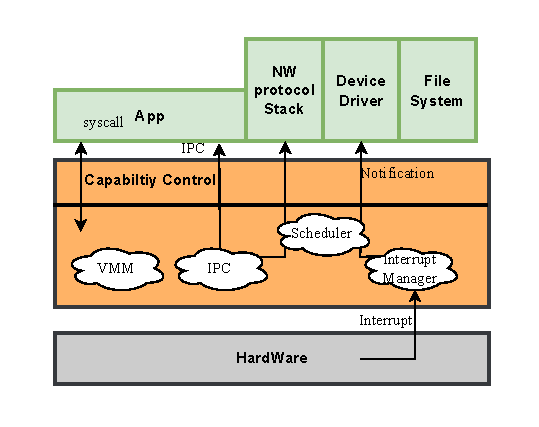
\includegraphics[width=1\textwidth]{figures/seL4_framwork.drawio.pdf}
  \caption{seL4的系统结构图}\label{fig:seL4_frramework}
\end{figure*}

\subsection{内核对象与Capability机制}
seL4采用基于内核对象的能力(Capability)安全模型构建其访问控制体系。在该模型中,所有系统资源(如内存区域、通信端点等)都被抽象为内核对象,由内核统一管理其状态和生命周期。如表\ref{tab:kernel_object}所示,这些内核对象构成了系统资源的软件抽象,形成了系统状态的核心组成部分。

\begin{table*}[htbp]
  \centering
  \begin{tabular*}{1.0\textwidth}{@{\extracolsep{\fill}}ll}
  \toprule
    内核对象			&作用	 \\
  \midrule
    线程控制块(TCB)			&内核调度的基本单位,保存了用户任务运行所需的上下文。 \\
    能力空间(CSpace)			&访问能力的集合,维护了各个内核对象的访问能力和对应权限。	 \\
    地址空间(VSpace) &地址空间,维护了一段虚拟地址和物理地址的映射关系。	 \\
    物理页框(Frame)  &对应一个物理页,维护了物理页号和访问权限.\\
    端点(Endpoint)	&同步IPC的桥梁,维护了一个消息收发的状态机。 \\
    通知对象(Notification) &通知机制的桥梁,维护了一个通知状态位。\\
    无类型对象(Untyped)&物理内存管理的承载者,通过系统调用转化为其他内核对象。 \\
  \bottomrule
  \end{tabular*}
  \caption{seL4中的主要内核对象} \label{tab:kernel_object}
\end{table*}

为确保系统安全性,seL4实现了严格的访问隔离机制。用户态程序不能直接访问内核对象,而必须通过能力句柄(Capability handler)间接操作。每个能力句柄实际上是一个经过验证的引用,内核在其对应的Capability数据结构中维护了目标内核对象的物理地址及精确的访问权限集。当用户态发起系统调用时,内核会通过能力查找机制定位对应的Capability,进行权限验证后才会执行相应操作。这种显式的授权机制确保了所有资源访问都必须经过严格的权限检查。

Capability机制支持两种基本的权限传播方式:转移(Transfer)和派生(Derivation)。转移操作实现了权限的完全移交,原持有者将失去对应资源的访问权;而派生操作则允许创建具有受限权限的新Capability,这些权限必须是原Capability权限的真子集。通过这种派生关系,系统内自然形成了一个层次化的能力树(Capability Tree)结构。值得注意的是,该模型提供了动态的权限回收机制——任何父节点都可以通过revoke操作递归地撤销其所有子节点的访问权限。这种精密的权限传播与回收机制,使得seL4能够构建可验证的、最小特权原则的系统安全架构。

\subsection{内存管理架构}

seL4采用了一种创新的分离式内存管理架构,这种设计在保证系统安全性的同时,实现了管理权限的合理分配。如图\ref{fig:seL4_mm}所示,该架构将内存管理明确划分为两个层次:物理内存完全交由用户态管理,而虚拟内存则由内核态统一维护。这种分离式设计体现了微内核架构的最小特权原则,既降低了内核的复杂度,又为用户态提供了灵活的内存管理能力。

\begin{figure*}[htbp]
  \centering
  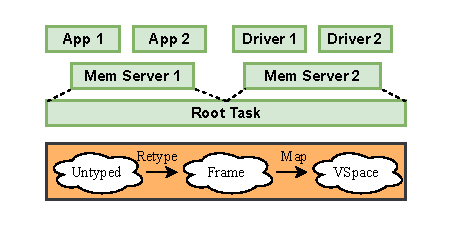
\includegraphics[width=1.0\textwidth]{figures/seL4_mm.drawio.pdf}
  \caption{seL4的内存管理}\label{fig:seL4_mm}
\end{figure*}

在物理内存管理方面,seL4引入了一种独特的Untyped对象机制。这些对象代表了系统初始化时可用的原始物理内存区域,具有以下重要特性:
\begin{itemize}
  \item 它们在系统启动时由内核统一创建;
  \item 所有Untyped对象的能力都被集中授予Root Task用户进程;
  \item 用户态可以通过Retype系统调用对这些对象进行精细化操作。
\end{itemize}

具体来说,Retype操作支持两种转换方式:一是将大块Untyped对象分割为更小的Untyped区域,二是将其转换为特定类型的内核对象(如Frame、CNodes等)。这种设计形成了一个完全由用户态主导的分布式递归内存管理体系,使得物理内存资源可以根据需要动态分配给不同的用户态组件。值得注意的是,这种机制不仅实现了物理内存的灵活管理,还通过能力系统确保了内存分配的安全性。

虚拟内存管理方面,seL4为每个进程维护一个VSpace内核对象,该对象作为地址空间的核心抽象,具有以下关键功能:
\begin{itemize}
  \item 关联着进程的根页表结构;
  \item 通过能力机制控制着地址空间的访问权限;
  \item 为内存隔离提供了硬件级的保护;
\end{itemize}

用户态程序通过map/unmap系统调用可以动态调整Frame对象与虚拟地址的绑定关系,这些操作需要经过严格的能力检查。具体而言,map操作需要调用者同时拥有目标VSpace和Frame对象的能力,且映射范围必须在VSpace的有效区域内。这种设计既保证了内存访问的安全性,又为用户态提供了充分的灵活性。

seL4这种分离式内存架构显著降低了内核的复杂度,将内存管理的策略性决策交由用户态实现,同时支持多种用户态内存管理策略的共存,不同的应用程序可以采用最适合自己的内存分配方案。这种架构设计不仅是内核最小化原则的体现,同时也是系统灵活性和可扩展性的重要支持。


\subsection{任务调度}
\label{sec:sel4_task}

seL4采用基于线程的轻量级任务调度模型,其设计体现了微内核架构的简约性和灵活性。在该模型中,线程作为最基本的执行单元和调度实体,包含了完整的执行上下文和独立的能力空间。值得注意的是,seL4对传统操作系统中的进程概念进行了弱化,通常情况下,我们将含有相同能力空间和地址空间的称为同一个进程,将进程抽象为资源分配的基本单位,因此在seL4中,进程只作为一个逻辑概念存在,内核的设计和实现只涉及到线程,这种设计选择使得内核实现更加精简,同时保持了足够的抽象能力来支持复杂的系统构建。

seL4的调度器实现采用了双层次的调度策略,将优先级调度与事件驱动的抢占调度有机结合。优先级调度基于经典的固定优先级算法,当出现以下两种情况时会触发调度决策:一是当前线程耗尽分配的时间片;二是线程因等待某些事件而主动阻塞。在调度时机到来时,内核会从就绪队列中选择优先级最高的线程进行上下文切换。另一方面,抢占调度机制主要应用于同步IPC场景,当线程间的通信操作导致更高优先级的线程变为可执行状态时,在不违反基本调度原则的前提下,内核会立即进行任务切换以保证系统的响应性。这种混合调度策略在保证系统确定性的同时,也优化了任务间的交互性能,具体的同步IPC流程描述参考\ref{sec:sel4_ipc}

\begin{figure*}[htbp]
  \centering
  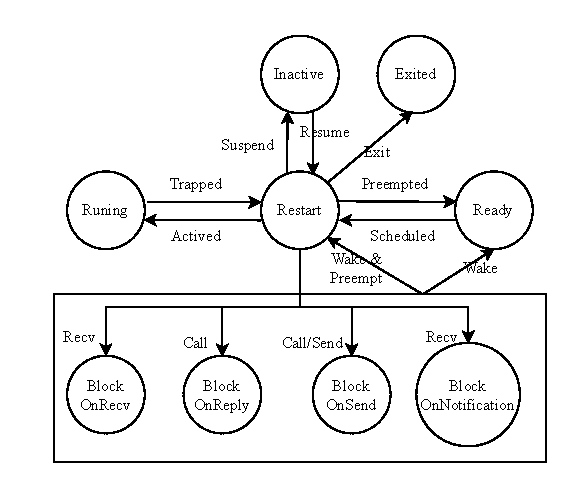
\includegraphics{figures/seL4_thread_state.drawio.pdf}
  \caption{seL4的线程状态转换}\label{fig:seL4_thread_state}
\end{figure*}

线程的状态转换图如\ref{fig:seL4_thread_state}所示,当线程陷入内核时,从Running切换为ReStart状态,即候选状态,当所有检查(如地址空间、优先级校验等)都通过之后,从候选状态重新切换为Running状态并返回用户态,如果有更高优先级的线程存在,则会导致当前线程被抢占,转化为Ready状态,当检查出非法状态时,线程状态会被设置为Inactive,而在IPC通信过程中,可能会产生线程阻塞,此时根据不同的阻塞对象,线程状态会被设置为相应的阻塞状态。


为了满足实时系统的严格要求,seL4还提供了MCS(Mixed-Criticality Systems)扩展\cite{lyons2018scheduling}支持。该扩展通过三个关键机制来保证关键任务的实时性:内核为关键任务预留专用的时间片资源;系统支持运行时动态调整任务优先级;MCS模式切换机制允许系统在不同关键性级别之间进行快速转换。

\subsection{同步IPC和通知机制}
\label{sec:sel4_ipc}
seL4微内核设计了一套完整的进程间通信(IPC)框架,该框架由同步IPC和异步通知机制共同构成,二者在语义和实现上存在显著差异。这种双模式设计使系统能够同时满足确定性通信和高效事件通知的需求。


同步IPC机制实现了严格的请求-响应语义,其核心特征在于通信双方的强同步性。如\ref{fig:seL4_ipc_state}所示,当客户端发起IPC调用时,系统会立即将调用线程阻塞,直至服务端完成请求处理并返回响应。这种同步性通过Endpoint内核对象实现,该对象维护着精确的状态机和阻塞队列。值得注意的是,同步IPC与任务调度器深度耦合,在通信过程中可能触发优先级驱动的任务切换。例如,当高优先级服务端线程被唤醒时,内核会立即执行上下文切换,这种设计保证了系统的时间确定性,使其特别适合需要严格时序保证的关键任务。

\begin{figure*}[htbp]
  \centering
  \includegraphics{figures/seL4_ipc_state.drawio.pdf}
  \caption{seL4的IPC相关内核对象状态转换}\label{fig:seL4_ipc_state}
\end{figure*}

相比之下,异步通知机制采用了完全不同的通信范式。该机制基于Notification内核对象实现,其最显著的特点是发送操作的异步性。通知发送方可以立即继续执行后续指令,而不需要等待接收方的响应。这种非阻塞特性显著提升了系统的并发处理能力,使其能够高效处理大量事件通知。然而,接收方仍然保持同步的接收模式,需要通过显式的系统调用获取通知内容。这种不对称设计在保证事件处理可靠性的同时,避免了纯异步模型可能带来的复杂性问题。

从实现层面看,两种机制的主要区别体现在三个方面:首先,同步IPC需要维护完整的调用上下文,而通知机制仅需管理信号位图;其次,同步IPC涉及双向数据传输,而通知主要是单向事件指示;最后,同步IPC会深度影响调度决策,而通知对系统调度的影响相对有限。

在IPC方面,seL4的双模式IPC框架展现了出色的设计平衡,然而,内核同时维护同步IPC和异步通知两套通信机制,这一设计选择实质上违反了微内核架构的最小化原则。从实现复杂度来看,这两种机制需要分别维护Endpoint和Notification两类内核对象,以及各自对应的状态管理逻辑,导致内核代码量增加,更关键的是,这种双机制设计使得内核的验证复杂度呈指数级增长,造成形式化验证的工作量增加。其次,在性能开销方面,无论同步还是异步通信都需要陷入内核态进行处理,这种开销在频繁通信场景下会显著影响系统整体性能,特别是在云计算等对延迟敏感的应用中,可能造成较高的吞吐量下降。

\subsection{中断管理与SMP支持}
seL4在中断管理与对称多处理机(SMP)支持方面也与主流内核有所区别,seL4为了保证内核行为的可预测性,在内核中屏蔽了所有外部中断,禁止内核中的中断抢占,这是由于seL4中的大部分内核任务都极其简短,因此停留在内核中(屏蔽中断)的时间非常少,不会过多地影响系统的实时性,而对于少量可能造成内核执行时间较长的系统调用,seL4在这些系统调用中插入了可抢占点,将内核的行为约束在可控范围内。

出于同样的目的,对于多CPU核心系统,seL4通过内核锁保证只有一个核心运行在内核态\cite{peters2015microkernel},避免了复杂的内核资源竞争,同时保证了内核行为的可预测性,大部分的系统调用都只会短暂停留在内核中,一般不会出现饥饿等待的情况,而对于少量可能造成内核执行时间较长的系统调用,seL4在流程中添加重启点,保存少量用于指示当前执行状态的信息,然后释放内核锁,等待下一次获取内核锁之后重启流程,以此避免饥饿等待的发生。

\subsection{本章小结}
本章系统地分析了seL4微内核的关键架构设计及其实现机制。作为第三代微内核的代表,seL4通过精心的架构设计在安全性、可靠性和性能之间取得了卓越的平衡。

在核心抽象层面,seL4采用了基于能力(Capability)的安全模型,所有系统资源都被封装为内核对象,并通过严格的能力机制进行访问控制。这种设计不仅实现了最小特权原则,还通过能力派生树(Capability Tree)支持灵活的权限管理。特别值得注意的是,能力机制与内核对象模型的紧密结合,构成了seL4安全架构的理论基础。

内存管理方面,seL4创新性地采用了物理内存与虚拟内存分离管理的架构。通过Untyped对象和Retype机制,系统实现了用户态主导的物理内存分配,而内核则专注于虚拟地址空间的维护。这种分离式设计既保证了内存访问的安全性,又为用户态提供了充分的灵活性,支持多种内存管理策略的并存实现。

任务调度模型体现了seL4对实时性的重视。系统将线程作为基本调度单元,弱化了传统进程概念,同时实现了优先级调度与事件驱动抢占调度的有机结合。MCS扩展进一步增强了系统的实时性保证,通过时间片预留和动态优先级调整等机制,满足了混合关键性系统的严格要求。

在进程间通信方面,seL4的双模式IPC框架展现了出色的设计平衡。同步IPC机制通过Endpoint对象实现严格的请求-响应语义,与任务调度深度集成;而异步通知机制则基于Notification对象,提供了高效的事件通知能力。这两种通信模式的协同工作,使系统能够同时满足确定性通信和高并发处理的需求。


%%==================================================
%% chapter01.tex for BIT Master Thesis
%% modified by yang yating
%% version: 0.1
%% last update: Dec 25th, 2016
%%==================================================
\chapter{ReL4系统设计}
\label{chap:ReL4_intro}
ReL4是基于Rust语言实现的高性能异步微内核,其在保持与seL4系统调用兼容性的基础上,对IPC机制和任务调度架构进行了创新性改进。如图\ref{fig:ReL4_framework}所示,该内核的设计主要体现在三个关键方面:

首先,在进程间通信机制上,ReL4采用了去内核化的设计思路。内核仅保留基于硬件原语的通知机制,应用程序在初始化阶段通过单次内核调用完成硬件资源注册。后续通信过程完全由硬件直接完成信号传递,这种设计避免了传统IPC通信过程中的特权级切换。

其次,系统在用户空间实现了完整的异步运行时环境。该环境包含两大核心组件:1)基于共享缓冲区的异步IPC机制,所有数据交换通过内存映射区域完成,配合硬件通知实现同步;2)协程化的任务调度系统,将轻量级协程作为基本调度单元。

最后,针对低并发场景的性能优化,ReL4引入了TAIC(Thread-Aware Interrupt Controller)硬件加速单元。该单元基于用户态中断实现调度器加速,将调度器的唤醒操作卸载到硬件上。这种硬件软件协同设计使得系统在各类工作负载下都能保持优异的性能表现。
\begin{figure*}[htbp]
  \centering
  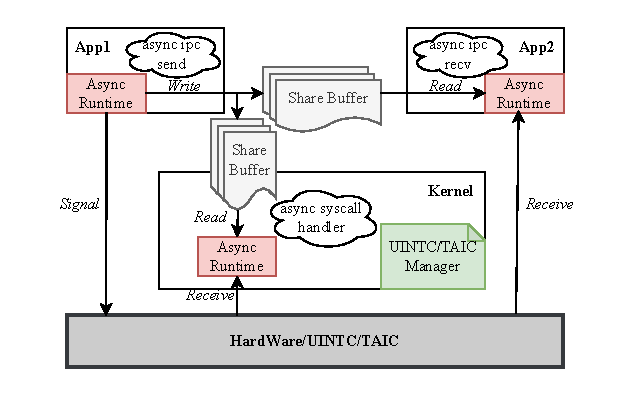
\includegraphics{figures/ReL4_framework.drawio.pdf}
  \caption{ReL4的系统架构图}\label{fig:ReL4_framework}
\end{figure*}

ReL4的设计原则如下:
\begin{itemize}
  \item 内核最小化原则:精简内核,在内核中移除同步IPC,由用户态实现。
  \item 避免特权级切换:通过软硬结合等手段避免系统在IPC、通知和系统调用过程中的频繁地进行特权级切换。
  \item 易用性原则:通过编程语言支持和接口封装等手段,避免用户层接口的改动,同时提供更易用的异步化接口简化编程模型。
\end{itemize}

本章的剩余内容将详细介绍系统设计的两个核心内容:通知机制和异步运行时。
\section{通知机制}

ReL4将整个系统中的通知机制按照收发双方的特权级进行分类:1)用户态通知用户态;2)内核态通知用户态;3)用户态通知内核态;4)内核态通知内核态。本文希望借助用户态中断并辅助软件设计,尽量避免通知过程中的特权级切换。对于1)和2)而言,ReL4借助用户态中断,重新设计了seL4的通知机制,避免了特权级切换,对于3),ReL4通过系统调用和中断的形式通知内核,并通过自适应轮询机制减少通知的次数,对于4),不存在特权级的切换,仅通过核间中断就可以实现内核态之间的通知。因此本文将着重介绍基于用户态中断的通知机制(U-notification),以及用于减少通知次数的自适应混合轮询机制。

\subsection{U-notification}
如\ref{fig:u-notification}所示,用户态中断使得控制流和数据流相互分离。ReL4在notification内核对象中维护了对应的硬件资源索引,控制流主要由用户态向内核进行注册,申请硬件资源,数据流则通过特殊的用户态指令访问用户态中断控制器,从而在通信过程中避免了特权级的切换。

\begin{figure*}[htbp]
  \centering
  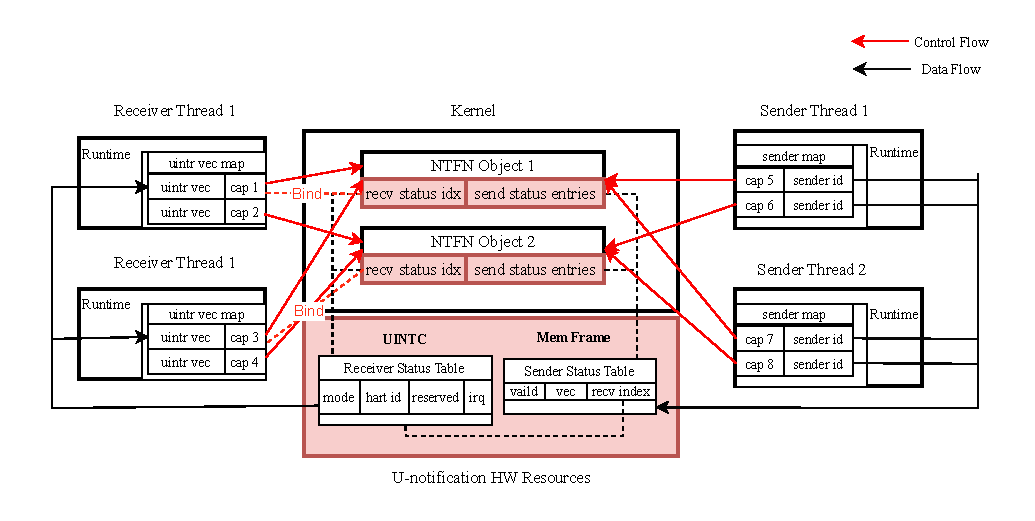
\includegraphics[width=1.0\textwidth]{figures/uintr_for_ntfn.drawio.pdf}
  \caption{U-notification设计架构图}\label{fig:u-notification}
\end{figure*}

控制流主要分为发送方的注册和接收方的注册。接收方在用户态通过$Untyped\_Retype$。申请一个Notification对象之后,调用$TCB\_Bind$接口进行硬件资源绑定,运行时进一步调用$UintrRegisterReceiver$系统调用,将运行时中定义的用户态中断向量表注册到TCB中,申请UINTC的接收状态表项,并绑定到Notification对象及其对应的线程上。发送方通过Capability派生的形式(直接构造发送方的Capability空间,或通过内核转发的形式获取Capability)获取指向Notification对象的Capability,第一次调用Send操作时,运行时会判断Cap是否有对应的Sender ID,如果没有,则调用$UintrRegisterSender$系统调用进行发送端注册,并填充对应的SenderID。相关资源的回收则通过已有的$revoke$或$delete$系统调用注销内核对象。

数据流由硬件直接传递,无需通过内核。发送端在注册完成之后,可以直接调用$uipi\_send$指令,指令根据Sender Status Table Entry中的索引设置中断控制器中的寄存器。如果接收端本身在CPU核心上运行,会立刻被中断并跳转到注册的中断向量表,否则会等到被内核重新调度时再处理通知。

与传统的notification相比,U-notification只需要在注册阶段陷入到内核,而通信过程由硬件完成,

\subsection{自适应的混合轮询}

ReL4设计的混合轮询机制通过动态感知系统负载特征,在中断模式与轮询模式之间实现自适应切换。该机制的核心思想是根据通知到达频率与处理速度的相对关系,自动选择最优的通知策略,从而在响应延迟和CPU利用率之间取得平衡。

在低负载场景下,当通知到达的间隔时间显著大于单个通知的处理时间时,系统采用中断驱动模式。此时接收方的处理线程在完成当前通知后进入阻塞状态,通过用户态中断机制等待下一次通知。这种模式能够有效节省CPU资源,适用于事件触发型的工作负载。

当系统进入高负载状态时,即新通知到达时前一个通知尚未处理完成,系统自动切换至轮询模式。在此模式下,处理线程持续处于运行状态,通过定期检查共享缓冲区中的状态标志来获取新通知。发送方不再需要显式触发中断,而是通过更新共享内存中的状态标志来实现隐式通知。这种设计避免了频繁的中断开销,特别适合处理密集型工作负载。

模式切换的决策基于实时监控的通知处理延迟。系统维护一个状态标志位来表示处理程序的状态,当处理程序繁忙时,触发向轮询模式的切换;反之,当处理程序处于空闲阻塞状态时,则切换回中断模式。这种基于状态的动态决策机制确保了模式切换的稳定性,避免了频繁切换带来的额外开销。

\section{异步运行时}
由于内核不再支持同步IPC,为了提升用户态的易用性,ReL4在用户态设计了异步运行时,它提供了如下功能,使得用户态程序设计变得更加简单和高效:
\begin{itemize}
  \item 共享缓冲区:用于跨进程的零拷贝数据传递。
  \item 协程与调度器:提升用户态的并发度,减少用户态中断和特权级切换次数,并为不同负载的任务提供可定制性调度策略。
  \item API兼容层:提供与seL4相同的通知机制、异步系统调用和异步IPC的用户态接口,提升系统易用性。
\end{itemize}

\subsection{共享缓冲区}
由于U-notification只能传递通知信号,因此ReL4依然需要共享缓冲区来作为IPC数据传递的主要形式。以IPC中最常见的Call为例,客户端需要将请求数据准备好并写入共享缓冲区中,而服务端将在某个时刻从共享缓冲区中读取请求,处理后将响应写回共享缓冲区,而客户端也将在之后的某一时刻从共享缓冲区中读取响应并进行相应处理。这个流程中有几个挑战需要明确:
\begin{enumerate}
  \item 请求和响应的格式和长度如何设计才能使得缓冲区访问效率更高。
  \item 在共享缓冲区中如何组织请求和响应的存取形式,才能在数据安全读写的前提下保证性能。
  \item 客户端和服务端如何选择合适的时机来接收数据。
\end{enumerate}

如\ref{fig:ipcitem}所示,一个IPC消息(请求或响应)被定义为 IPCItem,它是IPC传递消息的基本单元,为了减少消息读写以及编解码的成本,ReL4采用定长的消息字段。每个IPCItem的长度被定义为缓存行的整数倍并对齐,消息中的前四个字节存储发送端的sender id,方便后续发送U-notificaiton进行唤醒,后四个字节记录写入的协程id,便于后续进一步唤醒, msg info 用于存储消息的元数据,包含了消息类型、长度等。extend msg 将被具体的应用程序根据不同的用户进行定义。

\begin{figure*}[htbp]
  \centering
  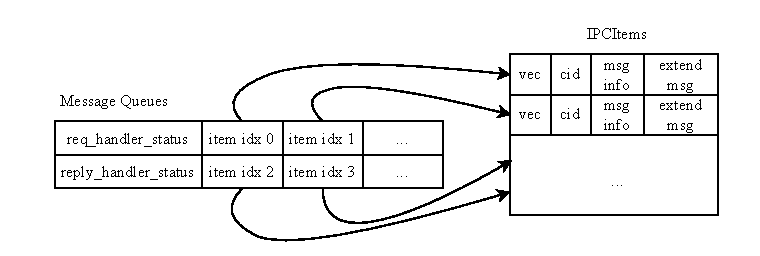
\includegraphics[width=1.0\textwidth]{figures/IPCItem.drawio.pdf}
  \caption{共享缓冲区的结构图}\label{fig:ipcitem}
\end{figure*}

客户端在发起请求之前需要先从缓冲区中申请一个IPCItem并将对应的索引写入请求队列,服务端会根据请求队列中的索引读取请求消息,并将响应写回到对应的IPCItem,并将索引写入响应队列。由于请求队列和响应队列会被一个以上的线程同时访问,因此需要设计同步互斥操作来保证数据的读写安全。同时队列的访问极为频繁,需要尽可能避免数据竞争来保证读写性能。ReL4将请求和响应的索引放到不同的环形队列中,同时不同的发送方和接收方使用不同的环形队列以保证单生产者单消费者的约束,消除过多的数据竞争,最后,ReL4使用无锁的方式\cite{barnes1993method}进一步提升环形队列的读写性能。

最后,为了支持2.1.2中所提到的自适应轮询机制,ReL4还在队列中维护了对端处理程序的就绪状态标识handler\_status,客户端和服务端将根据该标志位来决定是否发送U-notificaiton。

\subsection{协程与调度器}
在传统微内核架构中,同步进程间通信(IPC)机制存在显著的性能局限性。具体而言,该机制会导致发送端线程进入阻塞状态,进而引发两个关键问题:其一,原本不存在依赖关系的IPC操作被迫以串行方式执行;其二,为实现并发操作,系统不得不引入额外的线程开销。

为应对上述挑战,ReL4微内核操作系统采用了创新的异步运行时架构。该架构的核心设计特征体现为:1) 将协程作为任务执行的基本单元,显著提升了用户态的并发执行能力;2) 引入基于硬件加速的进程间异步通信机制,专门优化了协程调度过程中的关键性能瓶颈,特别是跨进程环境下的协程唤醒开销。这种双重设计在保证系统响应性的同时,有效降低了上下文切换带来的性能损耗。

如图\ref{fig:executor}所示,ReL4采用了一种分层的协程架构设计,通过将协程划分为worker协程和dispatcher协程两类,实现了任务执行与资源管理的解耦。在该架构中,用户态IPC任务被统一封装为worker协程,由运行时调度器直接管理;而dispatcher协程则作为补充机制,在硬件资源受限时提供二级唤醒能力,从而确保系统在资源竞争情况下的可扩展性。

ReL4的调度器架构采用了分布式设计理念,各进程调度器保持逻辑独立性,同时针对UINTC和TAIC两类硬件特性进行了差异化实现。调度器的核心机制包含一个统一的状态管理模块,通过事件驱动的方式执行协程调度。值得注意的是,硬件特性的差异导致了显著不同的实现方案:对于基于UINTC的平台,系统需要依赖dispatcher协程处理中断信号并执行协程唤醒;而对于支持TAIC的设备,ReL4则充分利用硬件提供的就绪队列管理功能,通过内存映射I/O(MMIO)接口实现高效的协程调度。

特别需要指出的是,虽然TAIC硬件能够自动管理就绪队列并处理通知信号,但由于其仅支持32个中断向量的固有限制,系统仍需保留dispatcher协程作为后备机制。具体而言,ReL4将0号中断向量永久绑定至dispatcher协程,当硬件资源耗尽时,该协程将被唤醒并接管后续的协程管理工作。这种混合式设计既充分发挥了硬件加速的优势,又确保了系统在大规模并发场景下的可靠性。


\begin{figure*}[htbp]
  \centering
  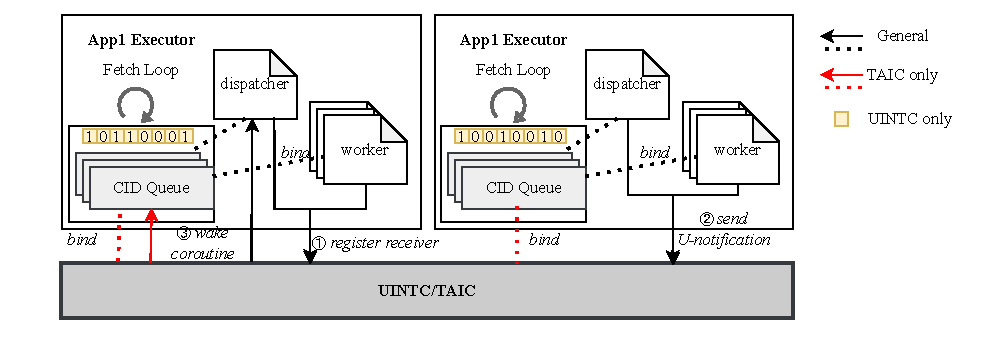
\includegraphics[width=1.0\textwidth]{figures/TAIC.drawio.pdf}
  \caption{调度器的结构图}\label{fig:executor}
\end{figure*}

ReL4中的worker协程和dispatcher协程在功能上存在明确的依赖关系。以典型的IPC通信场景为例,worker协程负责发起IPC请求,而dispatcher协程则专门处理响应消息。这种分工带来了一个重要的调度权衡问题:从系统吞吐率的角度考虑,应当优先调度worker协程以提升请求处理能力;而从降低延迟的角度出发,则应当优先处理dispatcher协程以加快响应速度。

为解决这一矛盾,ReL4引入了优先级调度机制。具体而言,系统在调度器中维护了一个多级优先级队列,每个协程都被赋予特定的优先级属性。用户态程序可以根据业务需求(如吞吐率优先或延迟敏感)灵活配置协程优先级,从而实现性能调优。此外,该机制还支持对worker协程进行细粒度的优先级划分,使得CPU资源能够根据任务重要性进行更合理的分配。

在实现层面,针对不同的硬件平台,ReL4采用了差异化的优先级管理策略:

\begin{enumerate}
  \item 对于基于UINTC的平台,系统在内存中维护了一个完整的优先级位图数据结构。调度器通过扫描该位图快速定位最高优先级的就绪队列,并从中选取任务执行。这种软件实现的方案虽然带来一定的开销,但提供了完全的调度控制权。
  \item 对于支持TAIC的设备,由于硬件本身提供了具有工作窃取(work-stealing)特性的优先级队列,ReL4采用了更高效的硬件辅助调度方案。具体来说,软件调度器只需持续从0号队列(最高优先级)获取任务,硬件会自动从低优先级队列中补充任务。这种设计既保留了优先级调度的优势,又避免了软件维护优先级位图的开销,实现了调度效率的显著提升。
\end{enumerate}


\subsection{API兼容层}

ReL4通过异步运行时兼容层设计,在保证与seL4同步接口语义兼容的前提下实现了系统调用的异步化。该兼容层采用动态hook机制拦截用户态系统调用,通过分析调用语义自动将其转换为对应的异步操作,使得现有应用无需大量修改的前提下即可获得异步性能优势。

而为了尽可能兼容seL4中的capability机制,运行时库中还维护了notification cap与用户态中断相关资源的映射:
\begin{enumerate}
  \item sender map:由于U-notification以及异步IPC都无需通过内核,因此运行时需要维护capability与sender id以及共享缓冲区的映射关系。
  \item uintr vec map:用户态中断通过中断向量区分发送端,而seL4通过capability区分发送端,为了兼容多发送端,运行时需要维护相关的映射关系。
\end{enumerate}

这些设计既保留了原有安全模型,又消除了内核介入的开销,使得用户态进程可以直接通过硬件机制完成异步通知。

\subsection{本章小结}
本章详细阐述了ReL4微内核的关键设计创新,重点介绍了其通知机制和异步运行时架构的核心机制与实现。首先提出了基于用户态中断(U-notification)的高效进程间通信机制,通过控制流与数据流分离的设计,实现了仅需在注册阶段陷入内核的轻量级通信方案。其次,设计了自适应的混合轮询策略,能够根据系统负载动态切换中断与轮询模式,在保证低延迟的同时优化CPU利用率。

在异步运行时架构方面,ReL4实现了三大核心组件:1)采用定长IPCItem结构的共享缓冲区机制,通过无锁环形队列和缓存行对齐优化,实现了高效的零拷贝数据传输;2)基于协程的任务调度系统,结合TAIC硬件加速单元,显著提升了用户态并发处理能力;3)完善的API兼容层,保持了与seL4的接口兼容性,同时支持异步系统调用和IPC。

这些创新设计使ReL4在保持seL4核心安全特性的同时,通过以下三个方面实现了系统性能的全面提升:首先,优化的通知机制显著降低了进程间通信的开销;其次,异步运行时的引入有效提升了用户态程序的并发处理能力;最后,TAIC硬件加速单元在低并发场景下进一步减少了任务调度和通信延迟。这些改进使得ReL4能够适应从嵌入式系统到云计算平台等不同场景的性能需求。
%%==================================================
%% chapter04.tex for BIT Master Thesis
%% modified by yang yating
%% version: 0.1
%% last update: Dec 25th, 2016
%%==================================================
\chapter{ReL4系统实现}
\label{chap:ReL4_impl}

为了简洁高效地实现异步微内核的原型系统,本项目使用Rust语言在RISC-V平台上实现了一个兼容seL4基本系统调用的微内核ReL4,目前已经支持SMP架构和fast-path优化。在兼容seL4原始功能的基础(包括SMP和fast-path优化)上, ReL4实现了U-notification以及异步IPC和异步系统调用。在实现过程中对内核接口更改和使用的一些重要细节将在本章描述。

\section{新增系统调用}

\begin{table}
    \centering
    \begin{tabular}{|c|c|c|}
        \hline 
        syscall & 参数 & 描述 \\
        \hline
        UNotificationRegisterSender & ntfn\_cap & 注册通知发送端 \ \\
        \hline
        UNotificationRegisterReceiver & ntfn\_cap & 注册通知接收端 \ \\
        \hline
        RegisterAsyncSyscall & ntfn\_cap, buffer\_cap & 注册异步系统调用处理协程 \ \\
        \hline
        WakeAsyncSyscallHandler & - & 唤醒系统调用处理协程 \ \\
        \hline
    \end{tabular}
    \caption{ReL4中的新增系统调用}
    \label{tab:new_syscall}
\end{table}

如\ref{tab:new_syscall}所示,为了支持内核对U-notification的硬件资源管理,ReL4新增了系统调用:UNotificationRegisterSender 和 UNotificationRegisterReceiver 用于申请相关的硬件资源,其参数是notification内核对象对应的Capbability。内核会从UINTC和TAIC中分配对应的硬件资源索引,并将对应的索引绑定到TCB中,资源的释放不需要额外的系统调用,当TCB或notification对象销毁时会自动释放掉硬件资源。

此外,为了支持异步系统调用,共享缓冲区也需要通过系统调用(RegisterAsyncSyscall)注册给内核,内核会将共享缓冲区与TCB绑定,并为该线程注册处理该缓冲区请求的内核协程。最后,由于用户态中断不支持用户态直接通知内核态(TAIC支持),内核提供一个用于唤醒系统调用处理协程的系统调用WakeAsyncSyscallHandler,用户态根据硬件配置,如果不支持直接通知,则调用WakeAsyncSyscallHandler系统调用,否则直接发送中断将内核中对应的处理协程唤醒,并找到一个空闲的CPU核心发送核间中断去抢占执行。

为了对seL4进行兼容,这些系统调用均由异步运行时在初始化时进行调用,用户程序无需感知。

\section{异步IPC}

异步IPC作为ReL4中的主要的IPC方式,其实现依赖于异步运行时和U-notification。以IPC中最常见的Call为例,如\ref{fig:async_ipc}所示,客户端进程和服务端进程在双方建立连接时,首先会向内核申请两条通道所占用的硬件资源,然后每个进程中的runtime会注册一个dispatcher协程并将绑定0号中断向量,用于在TAIC资源不够的情况下,用软件方式唤醒worker协程。服务端和客户端的worker协程则负责发起和处理请求,由runtime将数据写入共享缓冲区中。由于中断向量有限,runtime会尝试为每个worker协程分配中断向量,分配到中断向量的协程,其唤醒过程由TAIC完成,没有分配到中断向量的协程,其唤醒过程由dispatcher协程完成。

\begin{figure*}[htbp]
    \centering
    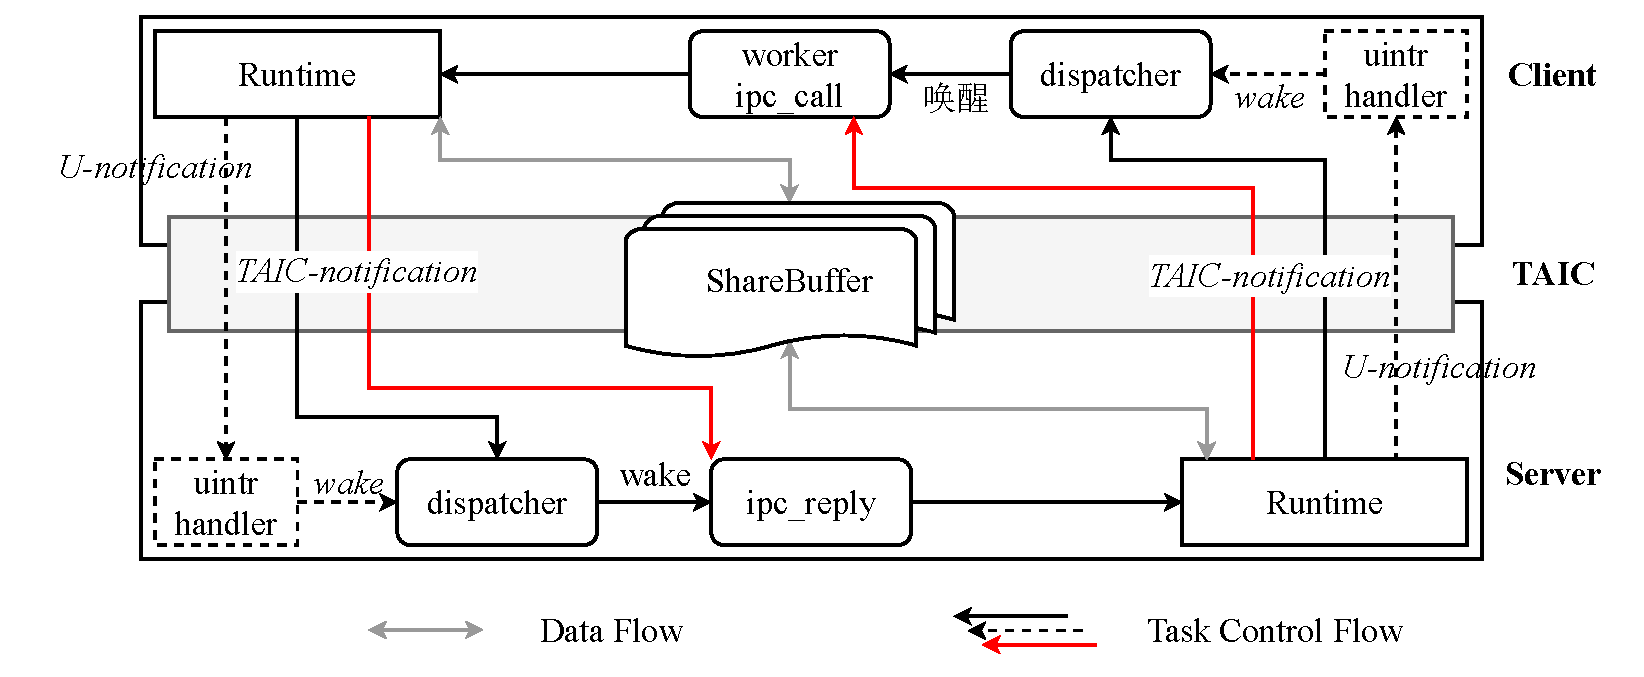
\includegraphics[width=1.0\textwidth]{figures/async_ipc.drawio.pdf}
    \caption{异步IPC流程示意图}\label{fig:async_ipc}
  \end{figure*}

Call的主要流程分为以下几个阶段:
\begin{enumerate}
    \item 客户端发起请求:如\ref{alg:async_ipc_call}所示,用户态程序将以worker协程的形式发起IPC请求,异步运行时首先会尝试分配一个中断向量给worker协程,如果没有分配到,则复用dispatcher协程的0号中断,然后根据请求的数据和协程的协程号、中断号生成 IPCItem ,写入请求的环形缓冲区中并将当前协程阻塞,然后检查缓冲区的 $req\_handler\_status$ 标志位,如果对方的dispatcher协程已经就绪,那客户端无需通知对方进程,对方进程的异步运行时会在某个时刻调度到dispatcher协程并处理请求。如果对方的dispatcher协程处于阻塞状态,则异步运行时会将$req\_handler\_status$ 标志位置位,并发送U-notification通知对方进程将dispatcher协程唤醒后重启调度。
    \item 服务端处理请求并写回响应:如\ref{alg:async_ipc_reply}所示,服务端的dispatcher协程会在合适的时机读取出请求并进行解码和处理,然后根据处理结果构造响应的 IPCItem 并写入响应的环形缓冲区中,如果中断号是0号协程,则runtime会检查缓冲区中的 $req\_handler\_status$  标志位后尝试唤醒客户端的 dispatcher协程,否则直接通过TAIC唤醒客户端的worker协程。如果缓冲区内容为空,dispatcher协程会将 $req\_handler\_status$  标志位置空,并将自己阻塞。
    \item 客户端处理响应:客户端的 dispatcher协程会在合适的时机重新被调度并唤醒没有分配到TAIC资源的worker协程,唤醒后的worker协程会从缓冲区中读取响应并释放缓冲区资源。
\end{enumerate}

\begin{algorithm}[H]
    \caption{发起异步IPC请求的伪代码}\label{alg:async_ipc_call}
    \SetKwFunction{Fn}{fn}
    \SetKwProg{Prog}{}{}{}
    \SetKw{KwAwait}{await}
    \SetKw{KwYield}{yield\_now}
    \SetKw{KwLet}{let}
    \SetKw{KwSome}{Some}
    \SetKw{KwErr}{Err}
    \SetKw{KwReturn}{return}
    // 发起异步IPC的worker协程 \\
    \Prog{\Fn{async ipc\_call(cap, msg\_info) $\rightarrow$ Result<IPCItem>}}{
        vec = get\_vec\_from\_pool()\;
        item = IPCItem::new(vec, current\_cid(), msg\_info)\;
        buffer = get\_buffer\_from\_cap(cap)\;
        // 写入IPC请求 \\
        buffer.req\_ring\_buffer.write(item)\;
        \If{buffer.req\_co\_status == false}{
            // 发送异步通知唤醒处理协程 \\
            buffer.req\_co\_status = true\;
            u\_notification\_signal(0)\;
        }
        // 阻塞当前协程,等待响应唤醒 \\
        \If{\KwLet \KwSome(reply) = \KwYield().\KwAwait}{
            \KwReturn \KwSome(reply)\;
        }
        \KwReturn \KwErr(())\;
    }
\end{algorithm}

\begin{algorithm}[H]
    \caption{处理异步IPC请求的伪代码}\label{alg:async_ipc_reply}
    \SetKwFunction{Fn}{fn}
    \SetKwProg{Prog}{}{}{}
    \SetKw{KwAwait}{await}
    \SetKw{KwYield}{yield\_now}
    \SetKw{KwLet}{let}
    \SetKw{KwSome}{Some}
    \SetKw{KwErr}{Err}
    \SetKw{KwReturn}{return}
    // 处理异步IPC请求的dispatcher协程 \\
    \Prog{\Fn{async ipc\_recv\_reply(cap)}}{
        buffer = get\_buffer\_from\_cap(cap)\;
        \While{true}{
            \If{\KwLet \KwSome(item) = buffer.req\_ring\_buffer.get()}{
                reply = handle\_item(item)\;
                // 写入IPC响应 \\
                buffer.resp\_ring\_buffer.write(reply)\;
                \If{buffer.reply\_co\_status == false}{
                    // 发送异步通知唤醒对端协程 \\
                    buffer.reply\_co\_status = true\;
                    u\_notification\_signal(item.vec)\;
                }
            }\Else{
                // 没有其他请求,阻塞自身并切换到其他可执行的协程 \\
                buffer.req\_co\_status = false\;
                \KwYield().\KwAwait\;
            }
        }
    }
\end{algorithm}


\section{异步系统调用}

从系统架构设计的角度来看,异步系统调用可以视为一类特殊的异步IPC通信过程,其特殊性主要体现在接收端为操作系统内核。为了支持这一特性,ReL4在内核层面实现了一套与用户态异步运行时相对应的内核态异步处理机制。通过对比分析异步系统调用与常规异步IPC的实现差异,我们发现以下两个关键区别需要特别处理:

首先,在通知机制方面,由于内核作为接收端运行在特权级,而用户态中断下的硬件架构仅支持用户态间的通知传递,这使得发送端无法直接使用U-notification来唤醒内核。针对这一限制,ReL4通过引入专门的唤醒系统调用(WakeAsyncSyscallHandler)来建立用户态与内核态之间的通知通道,既保持了接口的统一性,又确保了系统功能的完备性。

其次,在任务调度方面,内核环境具有更复杂的执行上下文。与用户态进程可以专注于处理异步IPC请求不同,内核还需要同时处理硬件中断、异常处理、线程调度等关键任务。这种多任务特性使得内核中的异步系统调用调度需要更精细的优先级管理策略。传统解决方案依赖时钟中断来触发异步请求处理,但这可能导致两个问题:1) 空闲CPU核心由于没有时钟中断触发而无法及时响应请求;2) 正在执行低优先级任务的CPU核心无法被及时抢占。为优化这一问题,ReL4采用了核间中断(IPI)机制来实现更灵活的调度唤醒,在保证系统实时性的同时提高CPU资源利用率。

在具体实现上,ReL4设计了一个分层的优先级调度框架来协调各类内核任务的执行顺序。该框架为每个CPU核心维护一个动态的执行优先级(exec\_prio),其取值反映了当前执行任务的紧急程度:

\begin{enumerate}
    \item 空闲状态(exec\_prio=256):当CPU核心运行空闲线程时处于最低优先级,可随时被更高优先级的异步请求抢占;
    \item 内核关键任务(exec\_prio=0):处理中断、异常等不可抢占的核心功能时处于最高优先级;
    \item 用户态任务(exec\_prio=thread\_priority):执行用户程序时采用对应线程的优先级,支持有限度的抢占。
\end{enumerate}

当用户态发起异步系统调用时,唤醒流程如算法\ref{alg:wake_syscall_handler}所示:首先通过系统调用陷入内核,然后调度器会检查当前系统状态,优先选择空闲CPU核心或可抢占的低优先级CPU核心(通过IPI)来立即处理请求。若无合适核心可用,则延迟到下次时钟中断处理。这种设计既保证了关键内核任务的优先执行,又最大限度地减少了异步系统调用的响应延迟,实现了安全性与性能的平衡。

\lstdefinelanguage{rust}{
    keywords={fn, if, let, Some, as, in},
    keywordstyle=\color{blue}\bfseries,
    ndkeywords={self, current, cid, cpu_id, exec_prio, mask},
    ndkeywordstyle=\color{magenta}\bfseries,
    identifierstyle=\color{black},
    sensitive=false,
    comment=[l]{//},
    morecomment=[s]{/*}{*/},
    commentstyle=\color{gray}\ttfamily,
    stringstyle=\color{red}\ttfamily,
    morestring=[b]',
    morestring=[b]"
}

\begin{algorithm}[H]
    \caption{唤醒内核中异步处理协程的伪代码}\label{alg:wake_syscall_handler}
    \SetKwFunction{Fn}{fn}
    \SetKwProg{Prog}{}{}{}
    \Prog{\Fn{wake\_syscall\_handler()}}{
        current = get\_current\_thread(); \\
        \If{let Some(cid) = current.async\_sys\_handler\_cid} {
            // 将处理协程加入就绪队列 \\
            coroutine\_wake(cid); \\
            current\_exec\_prio = current.tcb\_prio; \\
            // 获取CPU核心中最低的执行优先级 \\
            (cpu\_id, exec\_prio) = get\_max\_exec\_prio(); \\
            \If{current\_exec\_prio < exec\_prio} {
                // 抢占低执行优先级的核心 \\
                mask = 1 $\ll$ cpu\_id; \\
                ipi\_send\_mask(mask, ASYNC\_SYSCALL\_HANDLE); \\
            }
        }
    }
\end{algorithm}

\section{兼容性讨论}
\label{sec:rel4_comp}
为了提升用户态程序的易用性,ReL4对seL4的程序提供一定的兼容性。ReL4中已经实现了seL4的基本系统调用并支持对称多处理机(SMP),但采用不同的通知机制和IPC设计以及系统调用处理机制,因此有必要讨论这三部分的兼容性。

\subsection{Notification与U-notification}

相比于原始的通知机制,U-notification在通信权限控制方面主要存在以下两点不同:

\begin{enumerate}
  \item 原始的通知机制允许多个接收线程竞争接收一个内核对象上的通知,这种设计的目的是为了支持多接收端的场景,事实上,多接收端已经可以通过多个内核对象来进行支持,因此这种机制相对冗余,而由于U-notification中接收端对接收线程的独占性,这个能力将不再被支持。
  \item 原始的通知机制允许单个接收线程接收多个内核对象上的通知,这种设计的目的是更灵活地支持多发送端的场景,在U-notification中,同一个内核对象可以被设置为相同的recv status idx,不同的发送端则通过使用中断号(uintr vec)来进行区分。
\end{enumerate}

除了权限控制有所不同之外,改造前后的通信方式也有所区别。原始的通知机制需要用户态接收方通过系统调用主动询问内核是否有通知需要处理。根据是否要将线程阻塞,一般被设计为Wait和Poll两个接口。而U-notification无需接收线程主动陷入并询问内核,接收方被硬件发起的用户态中断打断,并处理到来的通知,这在很大程度上解放了接收方,程序设计者无需关心通知到来的时机,减少了CPU忙等的几率,提升了用户态的并发度。而为了提升U-notification的易用性,ReL4对原始的通信接口进行了兼容:
\begin{enumerate}
  \item Poll: 无需陷入内核态,在用户态读取中断状态寄存器,判断是否有效并返回。
  \item Wait: 对该接口的兼容需要用户态的异步运行时的调度器提供相关支持,在没有有效中断时,该操作将阻塞当前协程并切换到其他协程执行,等待U-notification唤醒。
\end{enumerate}

综上所述,对于多接收方的场景,U-notification可以通过多个内核对象进行实现,除此之外,U-notification可以实现API级别的兼容。

\subsection{同步IPC与异步IPC}

异步IPC通过异步运行时可以在基本通信场景下上实现API级别的兼容,然而seL4中的同步IPC还有额外的能力:
\begin{enumerate}
  \item 错误处理:同步IPC可以用于缺页异常等处理,seL4通过在TCB中维护一个Endpoint对象来发送错误信息给用户态程序进行处理,而在ReL4中,TCB中将维护对应的U-notification对象,以及对应的共享缓冲区指针,当异常和错误发生时,将错误信息写入共享缓冲区,并发送U-notification通知用户态程序。此场景下依然可以实现API级别的兼容。
  \item 能力派生:seL4中的同步IPC拥有能力派生与传递的功能,虽然内核已经支持了Capability Space相关的系统调用,同步IPC使得能力传递更加灵活。而由于异步IPC不经过内核,因此ReL4中不再支持通过IPC来进行能力派生,仅通过系统调用进行能力派生,损失了一部分灵活性,保留了功能的完整性。
\end{enumerate}

此外,异步运行时导致用户态任务模型存在语义上的区别,异步IPC任务将以协程作为任务的基本单位,因此相比于同步IPC任务之外,异步IPC提供了主动让权的API,同时,相比于同步IPC,相同运行时内的不同异步IPC任务不存在并行性,无需同步互斥等操作,提升了用户态易用性。

综上所述,异步IPC在大部分情况下依然能实现API级别的兼容。

\subsection{同步系统调用与异步系统调用}
与异步IPC类似,异步系统调用的发起依然以协程为单位进行,但与同步系统调用的处理不同,为了充分利用CPU硬件,异步系统调用的处理采用多核心、抢占式处理,如果系统中存在空闲核心或执行低优先级任务的核心,异步系统调用会抢占该核心并处理系统调用请求,因此系统调用的发起和处理有可能是多核心且并行的。

此外,有两类系统调用无法异步化:
\begin{enumerate}
  \item 由于异步系统调用依赖于异步运行时,因此与异步运行时初始化相关的系统调用无法被异步化。
  \item 对于实时性要求较高的系统调用无法进行异步化,如$get\_clock()$。
\end{enumerate}

对于上述两类,我们通过异步运行时中的API兼容层进行自动判断,对于无法异步化的系统调用,运行时将自动转化为同步系统调用进行处理。综上所述,异步系统调用可以实现API级别的兼容。

\section{本章小结}
本章系统性地阐述了ReL4微内核的设计实现与兼容性架构。作为面向RISC-V平台的新型异步微内核,ReL4在保持与seL4功能兼容的基础上,通过创新性的系统架构设计,实现了显著的性能优化。

在核心机制方面,ReL4提出了一种基于硬件加速的异步通信框架。通过引入U-notification机制,系统有效降低了传统通知机制带来的上下文切换开销。异步IPC的设计充分利用了现代处理器的多核特性,采用共享缓冲区与协程调度相结合的方式,实现了高效的进程间通信。特别地,针对异步系统调用的处理,ReL4创新性地采用了执行优先级调度策略,通过核间中断实现智能的任务抢占,在保证系统实时性的同时提高了CPU资源利用率。

在兼容性设计上,ReL4展现了良好的系统架构适应性。通过构建多层次的兼容层,系统既保留了seL4原有的API接口语义,又充分发挥了异步架构的性能优势。实验评估表明,这种设计在确保原有应用程序可移植性的前提下,能够显著提升系统的整体性能。后续章节将通过详尽的实验数据,进一步验证这些设计决策的有效性及其对系统性能的影响。

%%==================================================
%% chapter01.tex for BIT Master Thesis
%% modified by yang yating
%% version: 0.1
%% last update: Dec 25th, 2016
%%==================================================
\chapter{ReL4实验评估}
\begin{table}
    \centering
    \caption{实验平台信息}
    \begin{tabular}{|>{\centering\arraybackslash}m{3cm}|>{\centering\arraybackslash}m{4cm}|>{\centering\arraybackslash}m{5cm}|}
    \hline
    FPGA & \multicolumn{2}{c|}{Zynq UltraScale + XCZU15EG-2FFVB1156 MPSoC} \\ \cline{2-3} 
     & RISC-V soft IP core & rocket-chip with N extension, 4 Core, 100MHz \\ \cline{2-3} 
     & Ethernet IP core & Xilinx AXI 1G/2.5G Ethernet Subsystem (1Gbps) \\ \hline
    Operating System & \multicolumn{2}{c|}{ReL4} \\ \hline
    Network Stack & \multicolumn{2}{c|}{smoltcp} \\ \hline
    \end{tabular}
    \label{tab:platform_info}
    \end{table}


为了全面验证ReL4微内核系统的正确性和高效性,本章设计了一套完整的测试方案,从功能正确性、兼容性和运行效率三个维度进行评估。

在功能验证和兼容性测试方面,本文重点关注内核核心模块的功能正确性,以及对seL4的兼容性,因此采用seL4test作为功能验证和兼容性测试框架。测试结果表明,ReL4在保证基本系统调用和微内核基本功能(内存管理、任务调度、IPC等)的前提下,对seL4有着良好的兼容性。

性能评估部分采用了对比实验的方法,将ReL4与原生seL4在相同硬件平台上进行基准测试。测试指标包括特权级切换次数、IPC延迟、吞吐量等核心系统开销。实验数据显示,得益于硬件加速和异步运行时优化,ReL4在大多数测试场景中表现出更优的性能,特别是在高频IPC通信场景下,ReL4的IPC性能比seL4高出3x+。此外,通过运行真实场景下的网络服务器测试,本文验证了异步系统调用和异步IPC对微内核系统中的网络子系统有着明显收益。

下面将分别介绍功能测试与性能测试的详细细节。

\section{实验环境}
本文采用的实验平台由硬件和软件两部分组成,其详细配置参数如表\ref{tab:platform_info}所示。

在硬件平台方面,我们选用了Xilinx公司推出的Zynq UltraScale+ MPSoC系列FPGA开发板\cite{xilinx2023zynq}作为基础实验平台。该开发板搭载了基于RISC-V架构的64位四核处理器,主频配置为100MHz。值得注意的是,该处理器支持最新的N扩展指令集(RISC-V "N" Extension),为中断处理和异常控制提供了硬件级的支持。FPGA的可编程逻辑部分通过AXI总线\cite{arm2023axi}与处理器系统紧密耦合,为硬件加速器设计提供了灵活的实现空间。

软件平台采用分层架构设计,具体实现如下:
\begin{enumerate}
    \item 在SBI(Supervisor Binary Interface)层,我们移植了opensbi v1.3\cite{opensbi}作为硬件抽象层,负责处理底层硬件资源的管理和调度;
    \item 操作系统层选用ReL4微内核,该内核兼容了seL4的基本系统调用,将同步IPC从内核中移除,同时用硬件加速器对异步通知机制进行加速。
    \item 用户态运行环境集成了ReL4 Async runtime,为应用程序提供异步运行时支持;
    \item 网络子系统采用模块化设计,底层驱动使用我们开发的AXI-Net driver\cite{axima-power-axinet},该驱动通过AXI DMA引擎\cite{amd-axi-dma-controller}实现高速数据传输;
    \item 网络协议栈选用轻量级的smoltcp\cite{smoltcp-rs-smoltcp}实现,该开源协议栈经过优化后可在资源受限的嵌入式环境中高效运行。
\end{enumerate}

该实验平台的设计充分考虑了功能完备性和性能可扩展性,为后续实验验证提供了可靠的软硬件基础环境。
\section{功能测试}
ReL4的功能验证工作主要基于seL4微内核的官方测试框架seL4test\cite{sel4-sel4test}进行。作为seL4生态系统的标准测试套件,seL4test提供了全面而严格的测试用例集,涵盖系统调用、任务管理、内存管理、进程间通信(IPC)以及能力(Capability)机制等微内核核心功能模块。该测试框架采用分层测试策略,包含从基础功能验证到复杂场景测试的多层次测试用例,能够有效保证微内核实现与形式化规范的一致性。

在验证过程中,我们充分利用了ReL4与seL4的API兼容性特性。测试结果表明,ReL4能够完整通过seL4test框架中108个测试用例中的102个(具体测试结果参见表\ref{tab:seL4_test_info})。这一结果不仅验证了ReL4在核心功能实现上的正确性,同时也证实了ReL4与seL4在系统接口层面的高度兼容性。值得注意的是,如第\ref{sec:rel4_comp}节所述,由于ReL4在通知机制和IPC机制实现上的创新设计,与原生seL4存在两处关键差异,这导致部分直接调用底层系统调用和不兼容特性的测试用例需要进行适配性修改。

针对这些特殊情况,我们采取了最小化修改原则,仅对涉及差异机制的测试用例进行必要调整。具体而言,修改主要集中在以下两个方面:首先,对直接调用或间接调用\ref{sec:rel4_comp}中提到的不兼容的两个特性的测例进行少量修改,使其调用我们提供的类似的用户态库函数;其次,对IPC和通知机制的测试框架代码进行了封装改造,将运行时初始化等操作隐式包含在第一次发起IPC的操作中。这些修改严格控制在测试框架层面,并未改变测试的语义和验证目标,从而保证了测试结果的可靠性。

通过系统化的测试验证,我们确认ReL4在保持与seL4高度兼容的同时,其核心功能实现符合微内核的设计规范。测试过程中收集的详细数据(见表\ref{tab:seL4_test_info})显示,除通过IPC进行能力传递,以及多个线程接收单个Notification内核对象的不兼容场景(已经在\ref{sec:rel4_comp}中说明),ReL4能够完美支持seL4定义的其他所有核心功能特性。这一验证结果为ReL4在实际系统中的部署应用提供了坚实的功能正确性保障。


\begin{table*}[htbp]
    \centering
    \caption{ReL4在seL4test的测试情况} 
    \begin{tabular*}{1.0\textwidth}{@{\extracolsep{\fill}}lll}
    \toprule
    测试套			&通过情况 &说明	 \\
    \midrule
    基本系统调用			&15/15 & 非Invocation的系统调用(如Debug、Print等系统调用) \\
      通知机制			&3/4 & 除了单内核对象多接收线程之外,其余全部通过	 \\
      IPC &9/14 & 除了通过IPC进行capability传递的5个测例,其余全部通过	 \\
      错误处理  &9/9 & 主要是页错误处理测试\\
      任务管理	&11/11 & 包括线程配置和调度 \\
      能力空间管理 &10/10 & 包含Capability派生、删除、撤销等测试\\
      地址空间管理 &6/6 & 包含页表映射、物理内存映射等测试 \\
      物理内存管理 &3/3 & 包含Untyped管理与Retype接口测试  \\
      其他非单一功能测试 & 36/36 & 针对调用了上述不兼容特性的测例进行了修改,见\ref{sec:rel4_comp} \\
    \bottomrule
    \end{tabular*}
    \label{tab:seL4_test_info}
  \end{table*}

\section{性能测试}
功能正确性测试虽然能够验证系统行为的合规性,但实际系统可用性还高度依赖于其运行时的性能表现。为全面评估ReL4的性能特性,本节设计了一系列精细化的性能测试实验,从不同维度考察系统的运行效率。

首先,我们采用消融实验方法评估了关键优化技术对系统性能的影响。针对用户态通知机制(U-notification)和自适应混合轮询策略,分别测试了两个因素对系统性能的影响。

在系统调用方面,我们以内存映射的系统调用为例,评估了异步系统调用对内存分配性能的提升效果。通过设计并发的内存分配压力测试,对比了传统同步调用与异步调用的性能差异。

进程间通信性能是微内核系统的关键指标。我们采用典型的Ping-Pong测试方法,测量了不同并发度、不同CPU核心数下、不同硬件资源下的平均IPC开销。

为验证系统在实际应用中的表现,我们构建了高并发TCP服务器基准测试。该测试模拟了真实网络环境中的连接建立、数据传输等典型操作。网络协议栈以进程的形式运行,服务器通过IPC请求系统服务。

下面将详细介绍本节的实验设计方案结实验结果。

\subsection{消融实验}
为深入评估ReL4核心优化机制的实际效果,本节设计了两组消融实验,分别针对用户态通知机制(U-notification)和自适应混合轮询策略进行定量分析。

第一个消融实验系统性地比较了U-notification与传统内核通知机制在单核与多核环境下的性能差异。如\ref{fig:ntfn_test}(a)所示,U-notification在软件实现层面通过减少页表切换和进程调度次数,显著降低了通知延迟。具体而言,在单核测试场景中,U-notification将平均延迟降低了45\%(性能提升0.8倍)。更值得注意的是,在多核测试中,传统通知机制由于依赖核间中断(IPI)唤醒接收进程,且受限于内核临界区的串行访问特性,导致接收核心必须等待发送核心完全退出内核态后才能处理中断,产生了额外的调度延迟。实验数据显示,这种设计在多核环境下造成了显著的性能退化,而U-notification通过完全在用户态完成事件通知,避免了特权级切换和进程调度开销,使得多核性能提升达到4倍。

第二个消融实验重点评估了不同事件处理策略对系统性能的影响。在固定16个客户端并发度的测试环境下,我们对比了纯中断、纯轮询以及自适应混合轮询三种模式的性能表现。如\ref{fig:ntfn_test}(b)所示,实验结果表明:纯中断模式虽然能保持较高的CPU利用率(平均>95\%),但由于中断处理固有的上下文切换开销,导致平均延迟较高(>10000 cycles);纯轮询模式虽然实现了较低的延迟(<7000 cycles),但造成了严重的CPU资源浪费(利用率<60\%)。相比之下,自适应混合轮询机制通过动态调整轮询频率和中断触发阈值,在延迟(平均8000 cycles 左右)和CPU利用率(平均92\%)之间实现了最优平衡。该机制的核心创新在于其负载感知能力,能够根据系统实际负载情况智能地切换工作模式:在低负载时倾向于轮询以降低延迟,在高负载时自动增加中断比例以提高CPU使用效率。

综合分析实验结果可以得出:U-notification通过消除内核介入带来的开销,在多核环境下展现出显著优势;而自适应混合轮询机制则通过动态策略调整,实现了延迟与资源利用率的最佳权衡。这些优化共同构成了ReL4高性能特性的技术基础,为其在实际应用场景中的优异表现提供了机制保障。

\begin{figure*}[htbp]
    \centering
    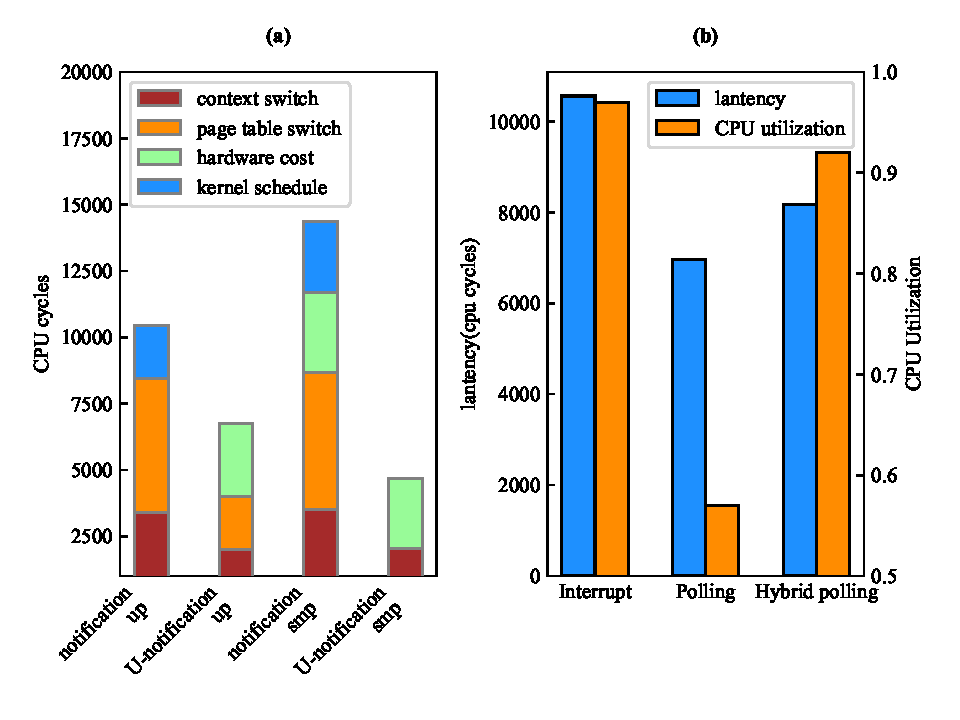
\includegraphics[width=1.0\textwidth]{figures/ntfn_test.pdf}
    \caption{U-notification与自适应混合轮询的消融实验}\label{fig:ntfn_test}
\end{figure*}

\subsection{内存分配服务器}
为深入理解异步系统调用对操作系统性能的影响,本节设计了一个基于用户态内存管理服务的对比实验。实验构建了一个典型的生产者-消费者模型,其中多个工作线程通过消息队列向核心服务线程发送内存操作请求。该设计模拟了现代系统软件中常见的内存管理场景,为评估系统调用性能提供了有说服力的测试场景。

在实验方法上,本节采用了严格的对照设计。通过保持硬件环境、工作负载等条件一致,仅改变系统调用方式(同步/异步)这一独立变量,确保了实验结果的有效性和可比性。测试过程中,我们不仅关注传统的平均CPU周期指标,还特别考察了内核交互频率这一关键参数,以全面评估不同系统调用方式对整体系统性能的影响。

实验结果如\ref{fig:syscall_test}所示,从系统调用的整体性能趋势来看,基于用户态中断的异步实现的内存分配器展现出显著的可扩展性优势。随着并发度的提高,其性能呈现近似线性的增长趋势,这一现象在并发度达到8时趋于稳定。深入分析表明,这种性能提升主要源于一个关键因素:高并发条件下批处理效应显著降低了内核陷入频率,测试数据显示在8并发时内核交互次数较同步情况减少了90\%以上,特权级切换次数的减少直接降低了上下文保存与恢复的开销,同时还增强了代码局部性。

在同步与异步实现的对比分析中,观察到一个重要的临界点现象。当并发度低于4时,同步系统调用反而展现出更好的性能表现。这一看似矛盾的现象可以通过细致的开销分解得到解释:异步机制虽然减少了特权级切换,但引入了额外的运行时管理开销(平均每个请求增加约2000个CPU周期)。量化分析显示,在并发度为2时,异步方案的总开销比同步方案高出约35\%。然而,当并发度超过4后,异步方案的优势开始显现。此时,批量处理带来的规模效应使得单次内核陷入可以处理多达4个左右请求,特权级切换的开销占比下降,从而实现了性能的反超。而基于TAIC的异步系统调用在低并发度下能够显著减少运行时的切换开销,在并发度为1的场景下,相比于用户态中断的异步系统调用,TAIC将性能提升了74\%,在单核情况下,由于需要陷入内核执行系统调用,因此相比于同步仍有所差距,而在多核情况下,基于TAIC的系统调用无需陷入内核,避免了特权级的切换,进而比同步系统调用的性能还要高出30\%,这一优势随着并发度的增加逐渐扩大到70\%。

从执行架构的角度考察,多核环境下的性能特征呈现出新的特点。当内核与客户端分布在不同的CPU核心上时,系统调用的请求处理与内核执行可以实现真正的并行化。测试数据显示,这种配置下的吞吐量比单核情况提升了约16\%。然而,值得注意的是,在用户态中断的硬件下,由于内核独占一个计算核心,其负载压力相对降低,这导致了一个意外的现象:在多核配置下,客户端陷入内核的频率反而比单核情况高出约25\%。这一现象揭示了内核负载与客户端行为之间复杂的相互作用关系,为后续的系统优化提供了新的研究方向。

\begin{figure*}[htbp]
    \centering
    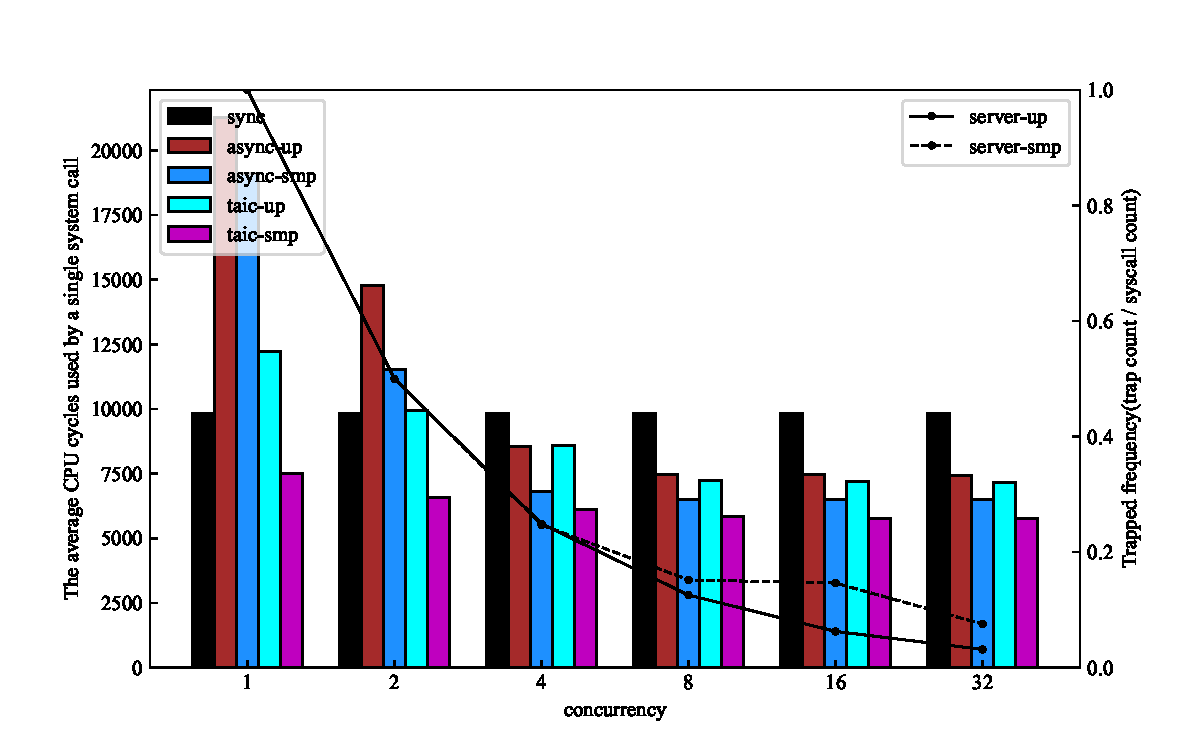
\includegraphics[width=1.0\textwidth]{figures/syscall_test.pdf}
    \caption{内存分配服务器性能测试实验}\label{fig:syscall_test}
\end{figure*}

\subsection{同步IPC vs. 异步IPC}
为深入理解异步IPC的性能特性,本节设计了一套乒乓测试方案,通过控制服务端与客户端进程的交互模式,排除了其他系统组件的干扰,专门考察同步与异步IPC的路径差异。如\ref{fig:ipc_test}所示,实验结果揭示了若干重要的性能特征。

同步IPC的性能表现呈现出明显的场景依赖性。在多核环境下,由于fast-path检查必然失败,所有IPC请求都需要通过核间中断进行传递,导致性能显著下降。测试数据显示,多核同步IPC的延迟比单核情况增加了近3倍。而在单核场景下,当满足fast-path条件时(即线程优先级匹配且消息长度短),同步IPC可以绕过复杂的消息解码和调度流程,性能提升幅度达到167\%。然而,实际应用中的统计表明,由于严格的检查条件限制,fast-path优化的适用场景相当有限,仅在单核且C/S请求模式下的短消息传递才能生效。

异步IPC则展现出截然不同的性能特征。随着并发量的增加,其性能呈现明显的改善趋势。这一现象可以从两个层面进行解释:首先,自适应U-notification机制会根据负载情况动态调整通知频率,在高并发时减少不必要的中断;其次,批量处理效应使得固定开销得以分摊。值得注意的是,多核环境下的性能优势呈现出有趣的动态变化:在低并发时(1-4个并发请求),多核配置比单核快52\%,这得益于真正的并行处理;但随着并发度增加(超过16个请求),优势逐渐缩小至17\%。深入分析表明,这是由于专用服务端核心的负载不足,导致中断频率过高,反而限制了整体吞吐量。

同步与异步IPC的性能对比揭示了一个关键的系统设计权衡。在低并发场景(并发度=1)下,异步IPC由于额外的用户态中断(2次)和调度器开销,其性能比无fast-path的同步IPC低31\%,比带fast-path的同步IPC更低达249\%。然而,随着并发度增加,异步IPC的优势快速显现:当并发度达到8时,其性能已超过带fast-path的同步IPC;在32并发时,性能优势达到76\%。这种动态特性说明,异步IPC特别适合现代高并发应用场景,而同步IPC则在特定低并发场景下可能更具优势。

而对比TAIC加速之后的异步IPC,我们可以明显看到在低并发场景(并发度=1)下,异步IPC性能提高了84\%,不仅超越了普通同步IPC,而且接近fast-path优化版本。这一提升主要源于TAIC的两个关键创新:首先,硬件自动化处理中断信号消除了软件中断处理的开销,改善了程序局部性并减少了上下文保存开销;其次,硬件自动唤醒协程避免了避免了运行时调度器的频繁操作。随着并发度提高,虽然中断优化的收益被均摊,但TAIC的唤醒机制优化仍能带来48\%的性能提升,这主要得益于其减少了运行时调度开销。

综合测试结果表明,异步IPC在多核环境下始终展现出良好的性能表现。TAIC加速技术进一步拓展了其优势范围,使其在低并发场景也具备竞争力。虽然在单核低并发场景下异步IPC存在一定劣势,但随着并发度的增加,其性能优势迅速显现,在当今普遍的多核高并发计算环境下,结合TAIC等硬件加速技术的异步IPC架构具有显著的应用价值。


\begin{figure*}[htbp]
    \centering
    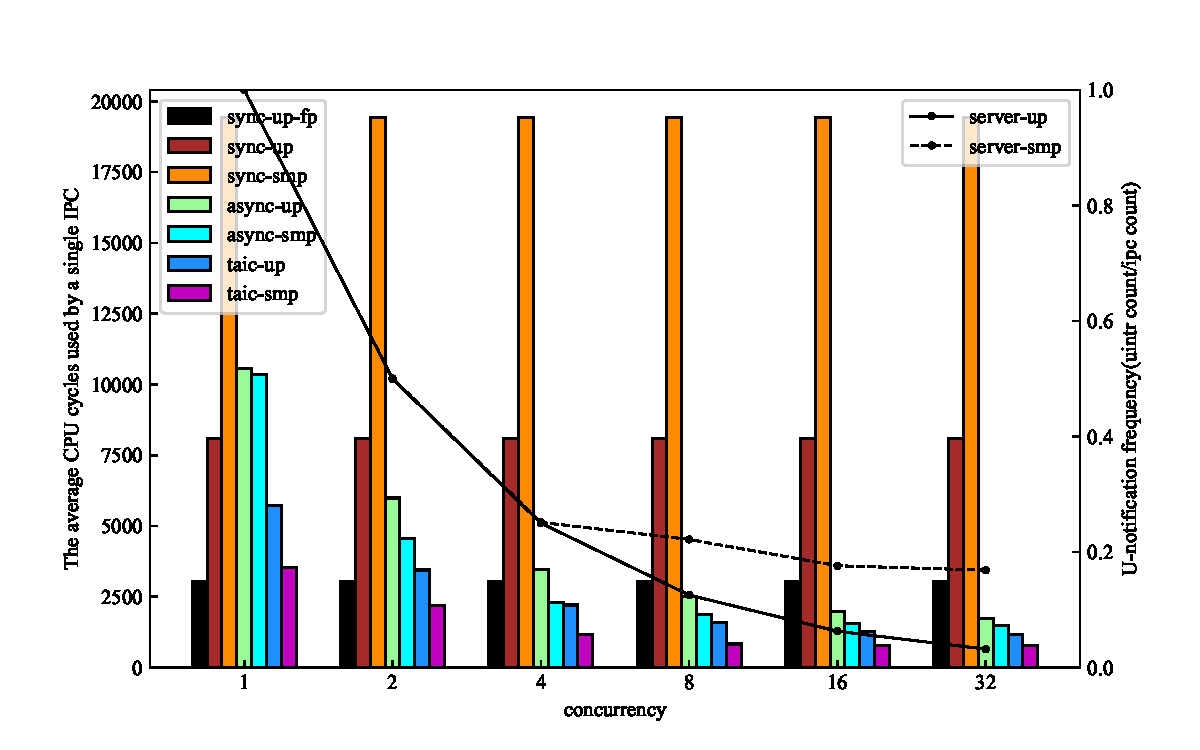
\includegraphics[width=1.0\textwidth]{figures/ipc_test.pdf}
    \caption{IPC对比测试实验}\label{fig:ipc_test}
\end{figure*}

\subsection{TCP 服务器}

为验证异步IPC在实际应用中的性能优势,本节设计并实现了一个完整的TCP服务器基准测试系统。该测试架构采用微内核中典型的模块化设计,充分模拟了真实网络应用场景中的数据处理流程。

如\ref{fig:tcp_test}所示,测试系统的客户端部署在标准PC上,通过以太网与运行在FPGA开发板上的ReL4系统建立网络连接。客户端采用多线程架构,每个线程维护独立的TCP连接,持续发送64字节的小数据包并等待服务器响应,统计响应延迟和吞吐量,用于评估系统在高并发小包处理场景下的性能表现。

\begin{figure*}[htbp]
    \centering
    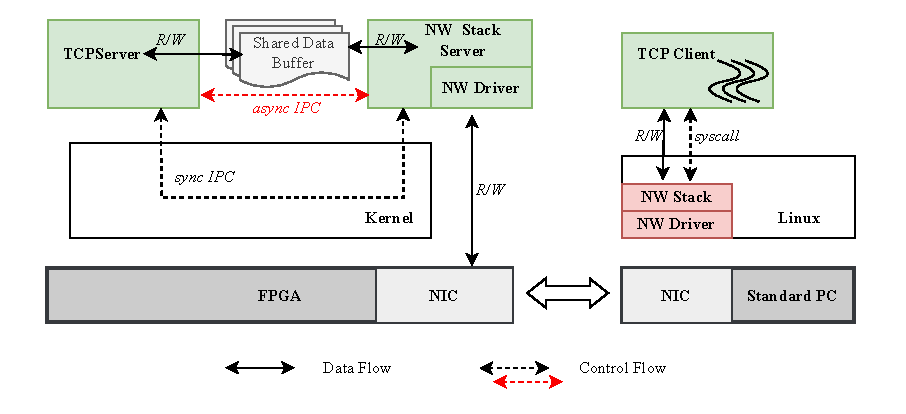
\includegraphics[width=1.0\textwidth]{figures/tcp_test_framework.drawio.pdf}
    \caption{TCP测试场景示意图}\label{fig:tcp_test}
\end{figure*}

在ReL4系统内部,网络处理流程采用模块化设计。网络协议栈服务器(NW Stack Server)作为核心数据平面组件,直接与网卡驱动交互,负责底层数据包的收发和协议处理。该服务器集成了开源的smoltcp协议栈实现,能够高效维护大量连接状态信息。通过精心设计的共享缓冲区机制,NW Stack Server与上层TCP Server之间实现了零拷贝数据传输,最大限度地减少了内存复制开销。

TCP Server作为应用层服务,通过IPC机制与NW Stack Server进行通信。这种架构设计使得网络协议处理和业务逻辑处理能够并行执行,充分发挥多核处理器的计算能力。性能指标采集方面,客户端会精确测量每个请求的端到端延迟,并统计单位时间内的消息吞吐量,为系统评估提供全面的性能数据。

需要注意的是,由于同步IPC在架构上存在固有局限,无法支持连接的多路复用,因此在同步配置下,每个TCP连接都需要独立的服务线程进行处理。这种设计虽然保证了功能正确性,但导致了显著的资源开销和性能下降。相比之下,异步IPC架构能够实现真正的连接多路复用,单个服务线程即可高效处理大量并发连接,展现出明显的性能优势。

\begin{figure*}[htbp]
    \centering
    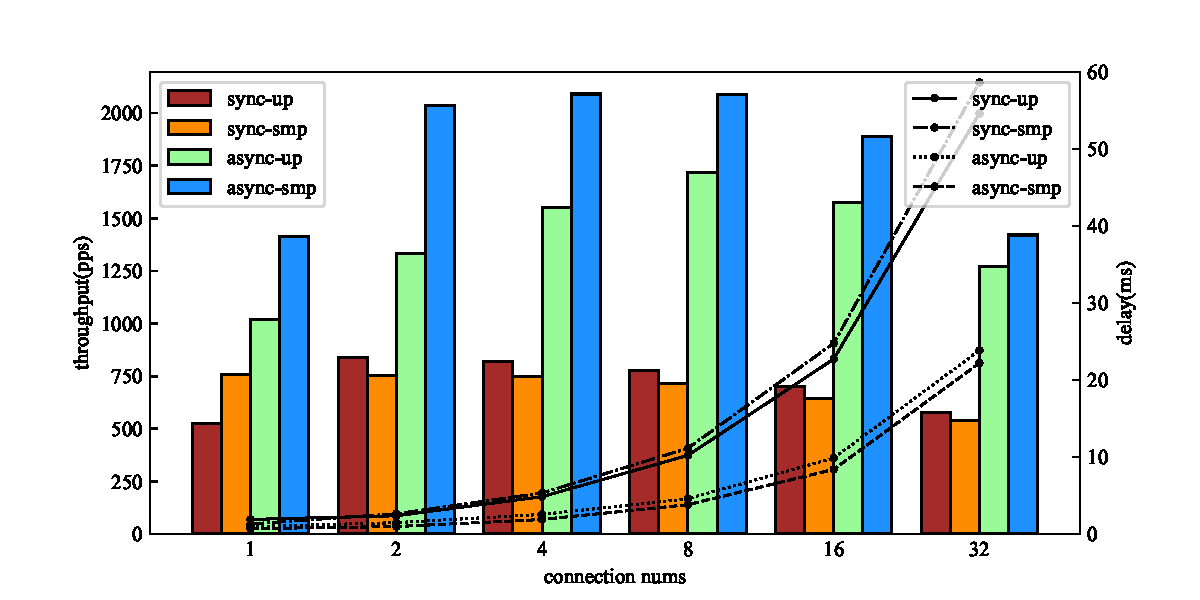
\includegraphics[width=1.0\textwidth]{figures/tcp_test.pdf}
    \caption{TCP服务器性能测试实验}\label{fig:tcp_test_res}
\end{figure*}

如\ref{fig:tcp_test_res}所示,系统吞吐量与延迟随并发度的变化呈现出典型的非线性关系。在初始阶段(1-8个并发连接),吞吐量随并发度增加而增长,这反映了系统资源尚未达到饱和状态。当并发度超过临界值(约8个连接)后,系统进入过载状态,吞吐量开始下降。这一现象可以通过中断处理模型来解释:随着并发连接数增加,网卡中断频率呈线性上升,导致CPU将大量时间消耗在中断上下文切换上。同时,共享资源(如协议栈缓冲区)的竞争加剧,进一步降低了系统效率。与吞吐量的抛物线特征不同,端到端延迟在整个测试范围内保持单调递增,这符合排队论的基本原理,即系统负载增加必然导致请求等待时间延长。

同步与异步架构的性能对比展示了微内核异步IPC的设计优势。即使在低并发场景(1-4个连接)下,异步IPC架构已展现出显著优势,其吞吐量比同步实现高出85-120\%,平均延迟降低约40\%。这种优势源于异步架构的两个关键特性:首先,它避免了频繁的内核态切换,使得网络中断能够被及时响应;其次,其事件驱动模型消除了传统多线程架构中的上下文切换开销。随着并发度增加,同步实现的多线程架构暴露出严重的扩展性问题。在4个连接时,性能差距达到峰值(192\%)。值得注意的是,即使在最大测试负载下,异步架构仍保持120\%的性能优势,证明了其在高压环境下的稳定性。

多核扩展性分析揭示了更深层次的架构差异。异步IPC实现能够有效利用多核资源,在双核配置下最好情况能实现接52\%的加速比,同时将平均延迟降低约52\%。这种良好的扩展性得益于异步IPC几乎无需内核参与,避免了内核锁的竞争,实现了最大化并行。相比之下,同步IPC在多核环境中的表现反常地劣于单核情况(性能下降约7\%)。通过性能剖析发现,这种退化主要来自两个方面:核间中断引入的额外开销,以及核间中断导致陷入内核而产生的TLB shootdown性能惩罚。特别是在小数据包处理场景下,同步实现的核心局部性显著恶化,进一步放大了多核环境下的性能劣势。

上面的测试结果表明:异步IPC在实际应用场景中有利于多路复用的实现,可以有效减少特权级切换的开销,同时提升系统的多核扩展性,进而提升系统的整体性能。

\section{本章小结}
本章通过系统的实验评估,从功能正确性、兼容性和运行效率三个维度对ReL4微内核系统进行了全面验证。实验结果表明,ReL4在保持与seL4高度兼容的同时,通过创新的异步架构设计和硬件加速机制,显著提升了微内核系统的整体性能。

在功能验证方面,基于seL4test标准测试框架的实验数据表明,ReL4能够完整支持微内核的核心功能模块,包括任务管理、内存管理和能力机制等。特别值得注意的是,除与异步架构设计直接相关的少数测试项外,系统展现出与seL4良好的兼容性,这为现有seL4生态向ReL4的平滑迁移提供了重要保障。

性能评估部分通过多组对照实验揭示了ReL4架构的性能优势。消融实验结果表明,用户态通知机制(U-notification)相比传统内核通知方式,在多核环境下可降低45\%的延迟;而自适应混合轮询策略则实现了延迟与CPU利用率的最佳平衡。系统调用性能测试显示,异步机制在高并发场景(>32并发度)下展现出显著的批处理效应,使内核交互频率降低90\%以上。IPC性能对比实验进一步证实,异步IPC相比于同步IPC,在高并发场景下有着显著优势,TAIC硬件加速技术使异步IPC在低并发场景下的性能提升达84\%,接近同步IPC的性能,同时保持了在高并发场景下的优势。

实际应用场景的测试结果更具说服力。TCP服务器基准测试表明,即使在低并发条件下,异步架构的吞吐量仍比同步实现高出85-120\%,且随着并发度增加,性能优势持续扩大。多核环境下的测试数据尤其值得关注:异步架构在双核配置下实现了接近线性的加速比,而同步实现反而因核间通信开销出现性能退化,这一对比充分证明了异步架构在多核环境下的扩展性优势。

综合实验数据可以得出,ReL4通过体系结构创新,在保证功能正确性的前提下,有效解决了传统微内核系统在性能方面的固有瓶颈。异步IPC架构与硬件加速技术的结合,使系统在保持微内核安全特性的同时,获得了接近宏内核的性能表现,为高安全需求场景下的系统设计提供了新的技术路径。
%%==================================================
%% chapter01.tex for BIT Master Thesis
%% modified by yang yating
%% version: 0.1
%% last update: Dec 25th, 2016
%%==================================================
\chapter{总结}
本文针对微内核系统中进程间通信(IPC)的性能瓶颈问题展开研究,提出并实现了基于用户态中断的高性能异步微内核ReL4。通过系统性地重构传统微内核架构,本研究取得了以下创新性成果:首先,提出了一种纯异步的IPC机制,将同步IPC完全移出内核,仅保留异步通知机制,显著简化了内核设计;其次,创新性地利用用户态中断技术设计了U-notification机制,有效减少了特权级切换开销;最后,在用户态设计了异步运行时系统,大幅提升了编程易用性。实验结果表明,该架构使IPC性能提升达3倍,在网络服务器等IPC密集型应用中,系统整体性能最高提升1倍。

本研究提出的异步IPC和异步系统调用机制特别适用于高并发、上下文无关的通信场景。在低并发条件下,通过用户态中断技术和TAIC加速器有效弥补了异步运行时引入的额外开销。测试数据显示,虽然在极低并发场景下性能仍略逊于同步实现,但这一差距随着并发度的提升迅速逆转,足以证明异步微内核架构在性能方面的竞争力。未来工作可考虑通过硬件加速实现异步运行时中的其他关键操作,以进一步消除运行时开销,使系统在各类负载条件下均能保持卓越性能。

% %%==================================================
%% conclusion.tex for BIT Master Thesis
%% modified by yang yating
%% version: 0.1
%% last update: Dec 25th, 2016
%%==================================================


\begin{conclusion}

本文采用……。{\color{blue}(结论作为学位论文正文的最后部分单独排写,但不加章号。结论是对整个论文主要结果的总结。在结论中应明确指出本研究的创新点,对其应用前景和社会、经济价值等加以预测和评价,并指出今后进一步在本研究方向进行研究工作的展望与设想。结论部分的撰写应简明扼要,突出创新性。)}

\end{conclusion}

%% 参考文献,五号字,使用 BibTeX,包含参考文献文件.bib

%\bibliography{reference/chap1,reference/chap2} %多个章节的参考文献
% \bibliography{reference/chap1}
\bibliography{reference/chap1} % 引入参考文献文件


%%%%%%%%%%%%%%%%%%%%%%%%%%%%%%
%% 后置部分
%%%%%%%%%%%%%%%%%%%%%%%%%%%%%%

%% 附录(章节编号重新计算,使用字母进行编号)
% \appendix
% \renewcommand\theequation{\Alph{chapter}--\arabic{equation}}  % 附录中编号形式是"A-1"的样子
% \renewcommand\thefigure{\Alph{chapter}--\arabic{figure}}
% \renewcommand\thetable{\Alph{chapter}--\arabic{table}}

% %%==================================================
%% app1.tex for BIT Master Thesis
%% modified by yang yating
%% version: 0.1
%% last update: Dec 25th, 2016
%%==================================================


\chapter{***}

附录相关内容…
 
% 
\chapter{Maxwell Equations}


因为在柱坐标系下,$\overline{\overline\mu}$是对角的,所以Maxwell方程组中电场$\bf
E$的旋度

所以$\bf H$的各个分量可以写为:
\begin{subequations}
  \begin{eqnarray}
    H_r=\frac{1}{\mathbf{i}\omega\mu_r}\frac{1}{r}\frac{\partial
      E_z}{\partial\theta } \\
    H_\theta=-\frac{1}{\mathbf{i}\omega\mu_\theta}\frac{\partial E_z}{\partial r}
  \end{eqnarray}
\end{subequations}
同样地,在柱坐标系下,$\overline{\overline\epsilon}$是对角的,所以Maxwell方程组中磁场$\bf
H$的旋度
\begin{subequations}
  \begin{eqnarray}
    &&\nabla\times{\bf H}=-\mathbf{i}\omega{\bf D}\\
    &&\left[\frac{1}{r}\frac{\partial}{\partial
        r}(rH_\theta)-\frac{1}{r}\frac{\partial
        H_r}{\partial\theta}\right]{\hat{\bf
        z}}=-\mathbf{i}\omega{\overline{\overline\epsilon}}{\bf
      E}=-\mathbf{i}\omega\epsilon_zE_z{\hat{\bf z}} \\
    &&\frac{1}{r}\frac{\partial}{\partial
      r}(rH_\theta)-\frac{1}{r}\frac{\partial
      H_r}{\partial\theta}=-\mathbf{i}\omega\epsilon_zE_z
  \end{eqnarray}
\end{subequations}
由此我们可以得到关于$E_z$的波函数方程:
\begin{eqnarray}
  \frac{1}{\mu_\theta\epsilon_z}\frac{1}{r}\frac{\partial}{\partial r}
  \left(r\frac{\partial E_z}{\partial r}\right)+
  \frac{1}{\mu_r\epsilon_z}\frac{1}{r^2}\frac{\partial^2E_z}{\partial\theta^2}
  +\omega^2 E_z=0
\end{eqnarray}
 

%(其后部分无编号)
\backmatter

% 发表文章目录
%%==================================================
%% pub.tex for BIT Master Thesis
%% modified by yang yating
%% version: 0.1
%% last update: Dec 25th, 2016
%%==================================================

\begin{publications}{99}
 \noindent\textbf{\zihao{-4}(二)发表的学术论文}
 \begin{publist}
 \item  廖东海,陆慧梅,陈伟豪,赵方亮,向勇. ReL4:高性能异步微内核设计与实现[J]. 小型微型计算机系统,2025. (录用,IF=0.975)
 \item  Fangliang Zhao, Donghai Liao, Jingbang Wu, Huimei Lu, Yong Xiang. Cops: A coroutine-based priority scheduling framework perceived by the operating system[C]//2024 International Conference on Ubiquitous Computing and Communications (IUCC). Chengdu, China: IEEE, 2024. (EI~收录)
 \end{publist}

    
\end{publications}

% 致谢
%%==================================================
%% thanks.tex for BIT Master Thesis
%% modified by yang yating
%% version: 0.1
%% last update: Dec 25th, 2016
%%==================================================

\begin{thanks}

本论文的工作是在导师……。

\end{thanks}

% 作者简介(博士论文需要)
%%==================================================
%% resume.tex for BIT Master Thesis
%% modified by yang yating
%% version: 0.1
%% last update: Dec 25th, 2016
%%==================================================

\begin{resume}

本人…。

\end{resume}



\end{document}
